% (c) 2014 Daniele Masini - d.masini.it@gmail.com
\chapter{Circonferenza}\label{chap:circonferenza}

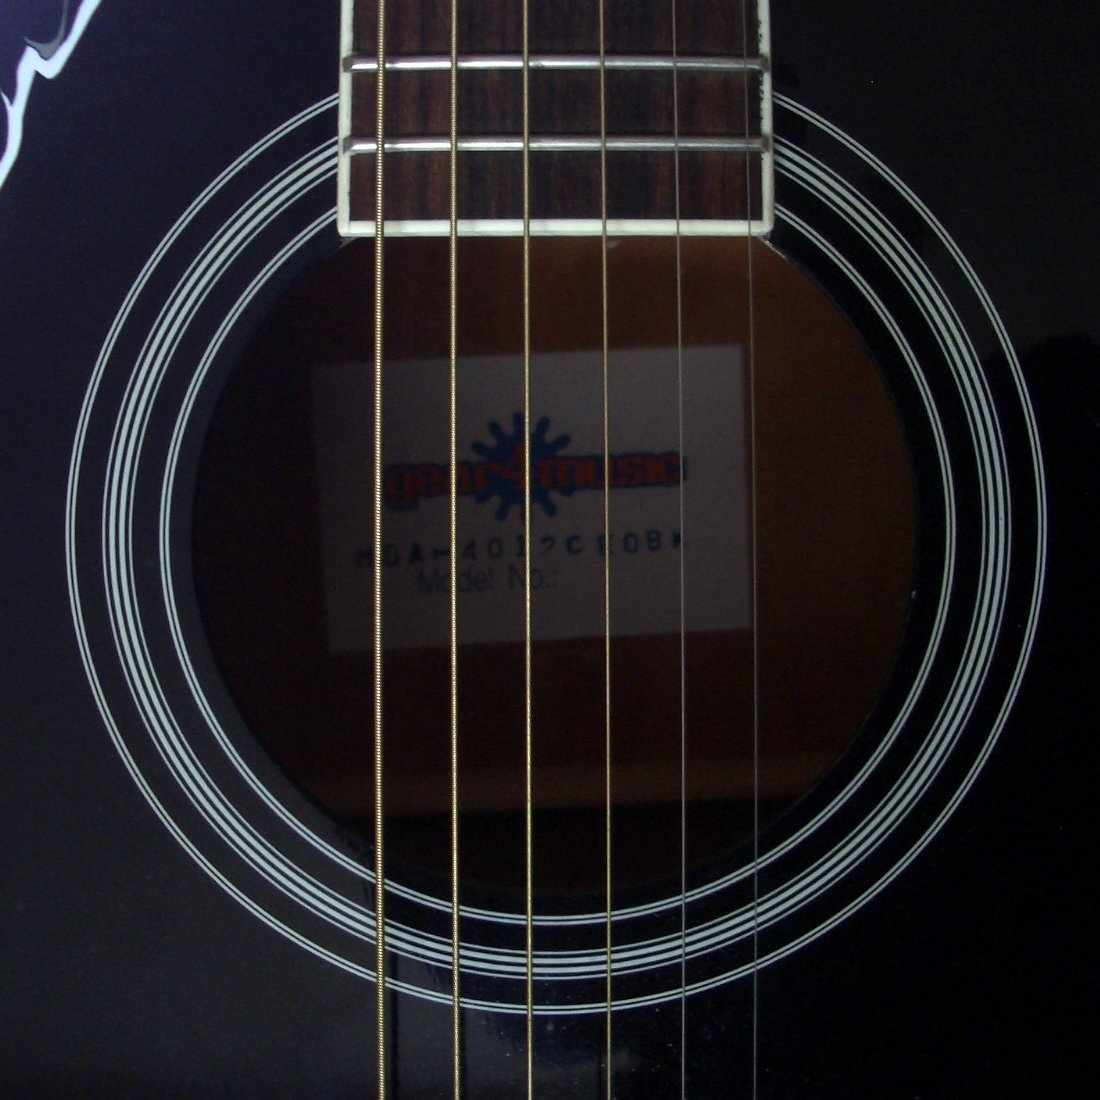
\includegraphics[width=0.95\textwidth]{circle.jpg}
  \begin{center}
    {\large ``Circle''}\par
    Foto di Howard Dickins\par
    \url{http://www.flickr.com/photos/dorkomatic/4551822855/}\par
    Licenza: Creative Commons Attribution 2.0\par
  \end{center}
\newpage

\section{Luoghi geometrici}

\begin{definizione}
Nel piano, si dice \emph{luogo geometrico} l'insieme di tutti e soli i punti del piano che verificano una proprietà, detta \emph{proprietà caratteristica} del luogo geometrico.
\end{definizione}
Ad esempio,
\begin{itemize*}
\item l'asse di un segmento è il luogo geometrico dei punti del piano equidistanti dagli estremi del segmento;
\item la bisettrice di un angolo è il luogo geometrico dei punti equidistanti dai lati dell'angolo.
\end{itemize*}
Se consideriamo la definizione ``costruttiva'' di asse di un segmento come retta perpendicolare al segmento stesso e passante per il suo punto medio, è possibile dimostrare che la nuova definizione di asse come luogo geometrico è ad essa equivalente.
Vale cioè il seguente
\begin{teorema}
Nel piano, il luogo geometrico dei punti equidistanti da due punti dati $A$ e $B$ è la retta $r$, perpendicolare al segmento $AB$ e passante per $M$, punto medio di $AB$.
\end{teorema}

\noindent\begin{minipage}{0.7\textwidth}\parindent15pt
Sia $r$ la retta perpendicolare ad $AB$ condotta da $M$, punto medio di $AB$. Dimostriamo che un generico punto $P\in r$ è equidistante da $A$ e $B$ e viceversa, un generico punto $Q$ tale che $QA\cong QB$ appartiene ad $r$.
~\\

\noindent Ipotesi: $r\perp AB$, $AM\cong MB$, $P\in r$.\tab Tesi: $PA\cong PB$.

\begin{proof}
Uniamo $P$ con $A$, $B$ ed $M$. Per ipotesi $PM \perp AB$, per cui, nel triangolo $PAB$, il segmento $PM$ è contemporaneamente altezza e mediana relative al lato $AB$; pertanto il triangolo $PAB$ è isoscele sulla base $AB$, da cui la tesi.
\end{proof}

\noindent Ipotesi: $QA\cong QB$ e $AM\cong MB$.\tab Tesi: $Q\in r$.

\begin{proof}
Uniamo $Q$ con $A$, $B$ ed $M$. Per ipotesi il triangolo $QAB$ è isoscele sulla base $AB$; inoltre il segmento $QM$ è la mediana relativa alla base del triangolo isoscele, per cui $QM$ è anche altezza. dunque la retta $QM$ coincide con la retta $r$, cioè l'asse di $AB$.
\end{proof}
\end{minipage}\hfil
\begin{minipage}{0.3\textwidth}
	\centering% Copyright (c) 2015 Daniele Masini - d.masini.it@gmail.com

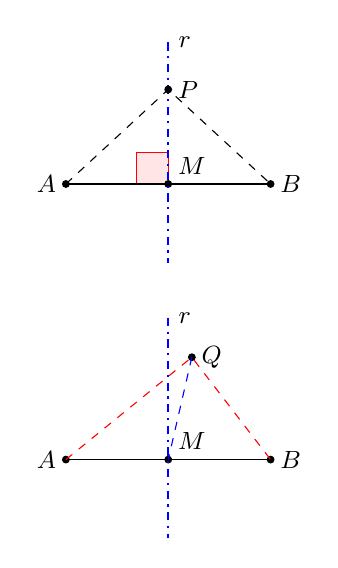
\begin{tikzpicture}[scale=1,font=\small]
\usetikzlibrary{calc}

\begin{scope}

\coordinate (a) at (-1.3,0);
\coordinate (b) at (1.3,0);
\coordinate (m) at ($(a)!0.5!(b)$);
\coordinate (p) at (0,1.2);

\draw[red, fill=red!10] (-.4,0) -- (-.4,.4) --(0,.4) -- (m);

\draw[fill] (a) circle (1.2pt) node[left] {$A$};
\draw[fill] (b) circle (1.2pt) node[right] {$B$};
\draw[fill] (m) circle (1.2pt) node[above right] {$M$};
\draw (a) -- (b);

\draw[blue, thick,dashdotted] (0,1.8) node[black,right] {$r$} -- (0,-1);
\draw[fill] (p) circle (1.2pt) node[right] {$P$};
\draw[dashed] (a) -- (p) -- (b);

\end{scope}

\begin{scope}[yshift=-3.5cm]

\coordinate (a) at (-1.3,0);
\coordinate (b) at (1.3,0);
\coordinate (m) at ($(a)!0.5!(b)$);
\coordinate (p) at (0,1.2);
\coordinate (q) at (0.3,1.3);

%\draw[red, fill=red!10] (-.4,0) -- (-.4,.4) --(0,.4) -- (m);

\draw[fill] (a) circle (1.2pt) node[left] {$A$};
\draw[fill] (b) circle (1.2pt) node[right] {$B$};
\draw[fill] (m) circle (1.2pt) node[above right] {$M$};
\draw (a) -- (b);

\draw[blue, thick,dashdotted] (0,1.8) node[black,right] {$r$} -- (0,-1);
\draw[fill] (q) circle (1.2pt) node[right] {$Q$};
\draw[dashed, red] (a) -- (q) -- (b);
\draw[dashed, blue] (q) -- (m);

\end{scope}

\end{tikzpicture}

\end{minipage}\vspace{5pt}

Analogamente, se consideriamo la classica definizione di bisettrice di un angolo come la semiretta interna all'angolo stesso avente origine nel suo vertice e tale da dividerlo in due angoli congruenti, possiamo dimostrare che la nuova definizione di bisettrice come luogo geometrico è equivalente a quest'ultima.
Vale cioè il seguente teorema.
\begin{teorema}
La bisettrice di un angolo è il luogo geometrico dei punti del piano equidistanti dai lati dell'angolo.
\end{teorema}

Sia $r\widehat{V}s$ un angolo (di vertice $V$ e di lati $r$ ed $s$) e sia $b$ la sua bisettrice (semiretta di origine $V$ che divide l'angolo a metà).
Verifichiamo prima che un generico punto $P\in b$ è equidistante da $r$ e da $s$.
~\\

\noindent Ipotesi: $P\in b$, $PK\perp s$, $PH\perp r$, $K\widehat{V}P\cong P\widehat{V}H$.\tab Tesi: $PK\cong PH$.\vspace{10pt}

\noindent\begin{minipage}{0.65\textwidth}\parindent15pt
\begin{proof}
Tracciamo da $P$ le perpendicolari ai lati dell'angolo e chiamiamo $H\in r$ e $K\in s$ i piedi delle due perpendicolari. Osserviamo che i triangoli $VPH$ e $VPK$, rettangoli rispettivamente in $H$ e $K$, risultano congruenti perché hanno rispettivamente congruenti l'ipotenusa e un angolo acuto, per i criteri di congruenza sui triangoli rettangoli risultano congruenti. Pertanto i cateti $PH$ e $PK$, opposti a $V$, risultano congruenti, da cui la tesi ($P$ equidistante da $r$ e da $s$).
\end{proof}
\end{minipage}\hfil
\begin{minipage}{0.35\textwidth}
	\centering% (c) 2014 Daniele Masini - d.masini.it@gmail.com
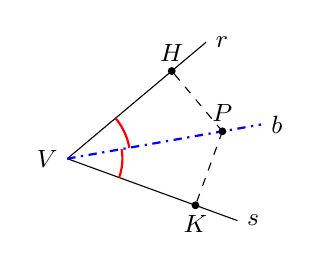
\begin{tikzpicture}[scale=1,font=\small]
\usetikzlibrary{calc}

\begin{scope}
\pgfmathsetmacro{\aalpha}{-20};
\pgfmathsetmacro{\abeta}{40};
\pgfmathsetmacro{\agamma}{(\abeta+\aalpha)/2};

\coordinate (o) at (0,0);

\coordinate (p) at ({\agamma}:2);

\draw (o) node[left] {$V$} -- ++({\aalpha}:2.3) coordinate (a) node[right] {$s$};
\draw (o) -- ++({\abeta}:2.3) coordinate (b) node[right] {$r$};
\draw[blue, thick, dashdotted] (o) -- ++({\agamma}:2.5) coordinate (c) node[right,black] {$b$};
\draw[fill] (p) circle (1.2pt) node[above] {$P$};
\draw[dashed] (p) -- ($(o)!(p)!(b)$) coordinate (h);
\draw[fill] (h) circle (1.2pt) node[above] {$H$};
\draw[dashed] (p) -- ($(o)!(p)!(a)$) coordinate (k);
\draw[fill] (k) circle (1.2pt) node[below] {$K$};

%\draw[thick,gray] ([shift=({\aalpha}:.5)]o) arc [radius=.5, start angle={\aalpha}, end angle={\abeta}];
\draw[thick,red] ([shift=({\abeta}:.8)]o) arc [radius=.8, start angle={\abeta}, end angle={\agamma}];
\draw[thick,red] ([shift=({\agamma}:.7)]o) arc [radius=.7, start angle={\agamma}, end angle={\aalpha}];
\end{scope}

\end{tikzpicture}

\end{minipage}\vspace{5pt}

Ovviamente, un qualsiasi punto appartenente ad una delle due semirette $r$ o $s$ che non sia il vertice $V$ non può essere equidistante da $r$ e da $s$, mentre il punto $V$ lo è (ha distanza nulla da entrambe).

Verifichiamo ora che, se $Q$ è un generico punto interno all'angolo $r\widehat{V}s$, se $Q$ è equidistante da $r$ e da $s$, deve risultare $Q\in b$.
~\\

\noindent Ipotesi: $QT\perp s$, $QL\perp r$, $QL\cong QT$.\tab Tesi: $T\widehat{V}Q\cong Q\widehat{V}L$.\vspace{10pt}

\noindent\begin{minipage}{0.65\textwidth}\parindent15pt
\begin{proof}
Infatti, se tracciamo da $Q$ le perpendicolari alle semirette $r$ ed $s$ e chiamiamo $L\in r$ e $T\in s$ i piedi delle perpendicolari, per ipotesi risulta $QL\cong QT$. Se uniamo $Q$ con $V$, si vengono a formare due triangoli rettangoli $QLV$ e $QTV$ con l'ipotenusa $QV$ in comune ed una coppia di cateti congruenti. Tali triangoli risultano pertanto congruenti per il quarto criterio (più semplicemente per il criterio particolare dei triangoli rettangoli), e di conseguenza $L\widehat{V}Q\cong Q\widehat{V}T$, per cui la semiretta $VQ$ coincide con la bisettrice $b$.
\end{proof}
\end{minipage}\hfil
\begin{minipage}{0.35\textwidth}
	\centering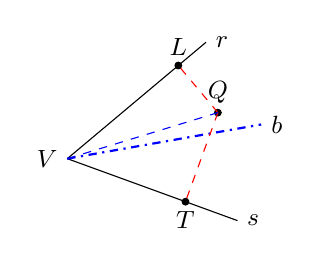
\begin{tikzpicture}[scale=1,font=\small]
\usetikzlibrary{calc}

\begin{scope}
\pgfmathsetmacro{\aalpha}{-20};
\pgfmathsetmacro{\abeta}{40};
\pgfmathsetmacro{\agamma}{(\abeta+\aalpha)/2};

\coordinate (o) at (0,0);

\coordinate (p) at ({\agamma}:2);
\coordinate (q) at ({\agamma+7}:2);

\draw (o) node[left] {$V$} -- ++({\aalpha}:2.3) coordinate (a) node[right] {$s$};
\draw (o) -- ++({\abeta}:2.3) coordinate (b) node[right] {$r$};
\draw[blue, thick, dashdotted] (o) -- ++({\agamma}:2.5) coordinate (c) node[right,black] {$b$};
\draw[fill] (q) circle (1.2pt) node[above] {$Q$};
\draw[dashed, red] (q) -- ($(o)!(q)!(b)$) coordinate (h);
\draw[fill] (h) circle (1.2pt) node[above] {$L$};
\draw[dashed, red] (q) -- ($(o)!(q)!(a)$) coordinate (k);
\draw[fill] (k) circle (1.2pt) node[below] {$T$};
\draw[blue, dashed] (o) -- (q);

%\draw[thick,gray] ([shift=({\aalpha}:.5)]o) arc [radius=.5, start angle={\aalpha}, end angle={\abeta}];
%\draw[thick,red] ([shift=({\abeta}:.8)]o) arc [radius=.8, start angle={\abeta}, end angle={\agamma}];
%\draw[thick,red] ([shift=({\agamma}:.7)]o) arc [radius=.7, start angle={\agamma}, end angle={\aalpha}];
\end{scope}

\end{tikzpicture}

\end{minipage}\vspace{5pt}


\section{Circonferenza e cerchio: definizioni e prime proprietà}

La definizione che ha dato Euclide di circonferenza fa riferimento ai luoghi geometrici: la circonferenza è il luogo geometrico dei punti del piano equidistanti da un punto del piano stesso, detto centro.
Intuitivamente, immaginiamo di fissare su di un piano un chiodo, di legare a questo chiodo una corda e di fissare all'altra estremità della corda una penna. Se facciamo ruotare la penna intorno al chiodo tenendo sempre in tensione la corda disegneremo una circonferenza.

\begin{definizione}
Assegnati nel piano un punto $C$ e un segmento $AB$, si chiama \emph{circonferenza} il luogo dei punti del piano che hanno distanza da $C$ congruente al segmento $AB$. Il punto $C$ viene detto \emph{centro} della circonferenza e la distanza dei punti della circonferenza dal centro è detta \emph{raggio} della circonferenza.
\end{definizione}

\osservazione Una circonferenza divide il piano in 3 insiemi:
\begin{itemize*}
\item l'insieme dei punti la cui distanza dal centro è minore del raggio. Questi punti si dicono \emph{interni} alla circonferenza.
\item l'insieme dei punti la cui distanza dal centro è uguale al raggio. Essi sono esattamente i punti della circonferenza.
\item l'insieme dei punti la cui distanza dal centro è maggiore del raggio. Questi punti si dicono \emph{esterni} alla circonferenza.
\end{itemize*}

Se consideriamo l'unione dell'insieme dei punti della circonferenza con l'insieme dei punti interni alla circonferenza otteniamo un cerchio.

\begin{definizione}
Chiamiamo \emph{cerchio} la figura formata dai punti di una circonferenza e dai punti interni ad essa.
\end{definizione}

Abbiamo definito la circonferenza come un insieme di punti tutti equidistanti dal centro. Viceversa osserviamo che il centro è l'unico punto del piano equidistante da tutti i punti della circonferenza. Per questo motivo possiamo affermare che una circonferenza è individuata esattamente dal suo centro e dal suo raggio o equivalentemente dal centro e da un suo punto.

\begin{definizione}
Un segmento che ha come estremi due punti distinti di una circonferenza è detto \emph{corda}. In particolare, una corda che contiene il centro della circonferenza viene definita \emph{diametro}.
\end{definizione}

I punti estremi di un diametro vengono detti \emph{diametralmente opposti}.
Ogni diametro è il doppio di un raggio e tutti i diametri della stessa circonferenza sono fra essi congruenti. Il centro della circonferenza è anche il punto medio di ciascun diametro.

Diamo ora alcune importanti proprietà delle corde.

\begin{teorema}
Il diametro è la corda di lunghezza massima.
\end{teorema}

\noindent\begin{minipage}{0.65\textwidth}\parindent15pt
\begin{proof}
Data una circonferenza di centro $O$ e raggio $r$, consideriamo una corda qualsiasi $AB$. Se essa passa per il centro $O$, coincide con il diametro e dunque $AB=2r$; altrimenti essa può essere considerata come la base di un triangolo isoscele $AOB$ avente come lati i due raggi $OA$ e $OB$. In tal caso per la disuguaglianza triangolare un lato di un triangolo è minore della somma degli altri due lati e dunque possiamo scrivere: $AB < OA + OB$ ovvero $AB < 2r$.
In conclusione, il diametro è maggiore di qualunque altra corda che non passa per il centro.
\end{proof}
\end{minipage}\hfil
\begin{minipage}{0.35\textwidth}
	\centering% Copyright (c) 2015 Daniele Masini - d.masini.it@gmail.com

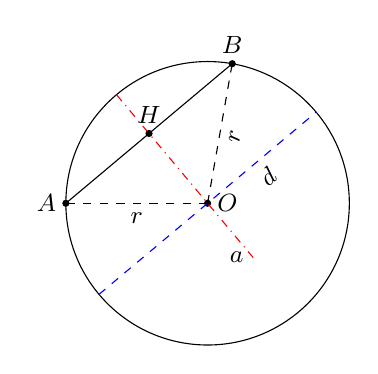
\begin{tikzpicture}[scale=.9,font=\small]
\usetikzlibrary{calc}

\begin{scope}
\pgfmathsetmacro{\aalpha}{-20};
\pgfmathsetmacro{\abeta}{40};
\pgfmathsetmacro{\agamma}{(\abeta+\aalpha)/2};

\coordinate (o) at (0,0);

\coordinate (p) at ({\agamma}:2);
\coordinate (q) at ({\agamma+7}:2);

\draw (o) circle (2);
\draw[fill] (o) circle (1.2pt) node[right] {$O$};

\draw[dashed] (o) -- node[below, midway, sloped] {$r$} (80:2) coordinate (b);
\draw[dashed] (o) -- node[below, midway, sloped] {$r$} (180:2) coordinate (a);
\draw[fill] (a) circle (1.2pt) node[left] {$A$};
\draw[fill] (b) circle (1.2pt) node[above] {$B$};
\draw (a) -- (b);
\path (o) -- (40:2) coordinate (d2);
\path (o) -- (40:-2) coordinate (d1);
\draw[blue, dashed] (d1) -- node[black, shift={(0.8,0)}, below, sloped] {$d$} (d2);
\path (o) -- (130:2) coordinate (o1);
\path (o) -- (130:-1) coordinate (o2);
\coordinate (h) at (intersection of o--o1 and a--b);
\draw[red, dashdotted] (o1) -- (o2) node[black, left] {$a$};
\draw[fill] (h) circle (1.2pt) node[above] {$H$};


\end{scope}

\end{tikzpicture}

\end{minipage}

\begin{teorema}
L'asse di una corda qualsiasi passa per il centro della circonferenza.
\end{teorema}

\noindent Ipotesi: $A$ e $B$ due punti distinti appartenenti alla circonferenza, $a$ asse della corda $AB$.\tab Tesi: l'asse passa per il centro della circonferenza.

\begin{proof}
Facendo riferimento alla figura precedente, poiché $OA$ e $OB$ sono raggi della circonferenza, il triangolo $AOB$ è isoscele sulla base $AB$. Ricordiamo che l'asse relativo alla base di un triangolo isoscele contiene l'altezza (nella figura $OH$). Dunque $O$ appartiene all'asse $a$ di $AB$.
Se la corda $AB$ coincide con un diametro, $O$ ne è il punto medio; ma poiché l'asse di un segmento è la retta perpendicolare al segmento stesso nel suo punto medio, in ogni caso l'asse passa per il centro $O$ della circonferenza.
\end{proof}

\begin{teorema}
Un diametro passante per il punto medio di una corda è perpendicolare alla corda stessa.
\end{teorema}

\noindent\begin{minipage}{0.65\textwidth}\parindent15pt
\begin{proof}
Il diametro passa per ipotesi dal punto medio $H$ della corda $AB$ e per definizione da $O$, centro della circonferenza nonché vertice del triangolo isoscele $AOB$. Dunque $OH$ è mediana del triangolo $AOB$ relativamente alla base $AB$. Per il teorema sul triangolo isoscele, la mediana relativa alla base di un triangolo isoscele è anche altezza e quindi essa è perpendicolare alla corda $AB$.
\end{proof}
\end{minipage}\hfil
\begin{minipage}{0.35\textwidth}
	\centering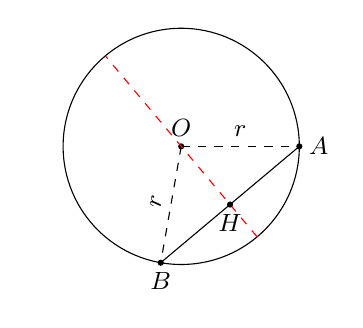
\begin{tikzpicture}[scale=.75,font=\small]
\usetikzlibrary{calc}

\clip (-2.6,-2.6) rectangle (2.6,2.01);
\begin{scope}[rotate=180]
\pgfmathsetmacro{\aalpha}{-20};
\pgfmathsetmacro{\abeta}{40};
\pgfmathsetmacro{\agamma}{(\abeta+\aalpha)/2};

\coordinate (o) at (0,0);

\coordinate (p) at ({\agamma}:2);
\coordinate (q) at ({\agamma+7}:2);

\draw (o) circle (2);
\draw[fill] (o) circle (1.2pt) node[above] {$O$};

\draw[dashed] (o) -- node[above, midway, sloped] {$r$} (80:2) coordinate (b);
\draw[dashed] (o) -- node[above, midway, sloped] {$r$} (180:2) coordinate (a);
\draw[fill] (a) circle (1.2pt) node[right] {$A$};
\draw[fill] (b) circle (1.2pt) node[below] {$B$};
\draw (a) -- (b);
\path (o) -- (130:2) coordinate (o1);
\path (o) -- (130:-2) coordinate (o2);
\coordinate (h) at (intersection of o--o1 and a--b);
\draw[red, dashed] (o1) -- (o2);
\draw[fill] (h) circle (1.2pt) node[below] {$H$};


\end{scope}

\end{tikzpicture}

\end{minipage}

\begin{teorema}
In una circonferenza, corde congruenti hanno eguale distanza dal centro (e viceversa).
\end{teorema}

\noindent\begin{minipage}{0.65\textwidth}\parindent15pt
\noindent Ipotesi:
\begin{itemize*}
\item $AB\cong CD$ (corde congruenti);
\item $OH\perp AB$ ($OH$ distanza della corda $AB$ dal centro $O$);
\item $OK\perp CD$ ($OK$ distanza della corda $CD$ dal centro $O$).
\end{itemize*}
\noindent Tesi: $OH\cong OK$.

\begin{proof}
Consideriamo triangoli isosceli $AOB$ e $COD$; essi sono congruenti per il 3\textsuperscript{o} criterio di congruenza poiché per ipotesi le basi $AB$ e $CD$ sono congruenti e i lati $AO$, $OB$, $OC$ e $OD$ sono tutti raggi della circonferenza.
Di conseguenza anche le altezze $OH$ e $OK$ sono congruenti.
\end{proof}
\end{minipage}\hfil
\begin{minipage}{0.35\textwidth}
	\centering% Copyright (c) 2015 Daniele Masini - d.masini.it@gmail.com

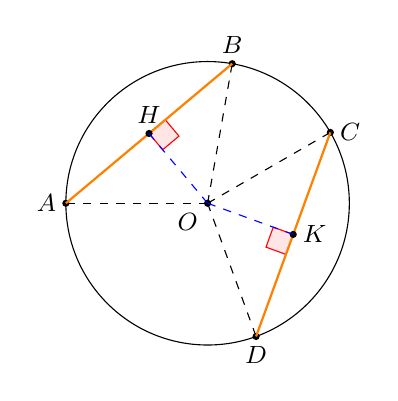
\begin{tikzpicture}[scale=.9,font=\small]
\usetikzlibrary{calc}

\begin{scope}
\pgfmathsetmacro{\aalpha}{-20};
\pgfmathsetmacro{\abeta}{40};
\pgfmathsetmacro{\agamma}{(\abeta+\aalpha)/2};

\coordinate (o) at (0,0);

\draw (o) circle (2);
\draw[fill] (o) circle (1.2pt) node[below left] {$O$};

\draw[dashed] (o) -- (80:2) coordinate (b);
\draw[dashed] (o) -- (180:2) coordinate (a);
\draw[fill] (a) circle (1.2pt) node[left] {$A$};
\draw[fill] (b) circle (1.2pt) node[above] {$B$};
\path (o) -- (130:2) coordinate (o1);
\coordinate (h) at (intersection of o--o1 and a--b);
\begin{scope}[rotate=40]
\draw[red,fill=red!10] (h) rectangle ([shift={(0.3,-0.3)}]h);
\end{scope}
\draw[thick, orange] (a) -- (b);
\draw[fill] (h) circle (1.2pt) node[above] {$H$};
\draw[dashed, blue] (o) -- (h);

\draw[dashed] (o) -- (30:2) coordinate (c);
\draw[dashed] (o) -- (-70:2) coordinate (d);
\draw[fill] (c) circle (1.2pt) node[right] {$C$};
\draw[fill] (d) circle (1.2pt) node[below] {$D$};
\path (o) -- (-20:2) coordinate (o2);
\coordinate (k) at (intersection of o--o2 and c--d);
\begin{scope}[rotate=70]
\draw[red,fill=red!10] (k) rectangle ([shift={(-0.3,0.3)}]k);
\end{scope}
\draw[thick, orange] (c) -- (d);
\draw[fill] (k) circle (1.2pt) node[right] {$K$};
\draw[dashed, blue] (o) -- (k);

\end{scope}

\end{tikzpicture}

\end{minipage}\vspace{8pt}

\noindent Viceversa\vspace{5pt}

\noindent Ipotesi:
\begin{itemize*}
\item $OH\cong OK$ (le distanze delle corde $AB$ e $CD$ dal centro $O$ sono congruenti);
\item $OH\perp AB$ ($OH$ distanza della corda $AB$ dal centro $O$);
\item $OK\perp CD$ ($OK$ distanza della corda $CD$ dal centro $O$).
\end{itemize*}
\noindent Tesi: $AB\cong CD$.

\begin{proof}
Consideriamo i triangoli rettangoli $AOH$ e $DOK$. $AO\cong DO\cong r$ (raggio della circonferenza) e $OH\cong OK$ per ipotesi; per il criterio particolare dei triangoli rettangoli, i due triangoli sono congruenti e quindi $AH\cong DH$. Allo stesso modo possiamo dimostrare che i triangoli rettangoli $BOH$ e $COK$ sono congruenti, per cui $BH\cong CK$. Dunque $AB \cong AH + BH \cong DK + CK \cong CD$.
\end{proof}

\begin{teorema}
Fra due corde disuguali, è maggiore quella che ha distanza minore dal centro (e viceversa).
\end{teorema}

\noindent Ipotesi:
\begin{itemize*}
\item $AB>CD$ (corde disuguali),
\item $OH\perp AB$ ($OH$ distanza della corda $AB$ dal centro $O$),
\item $OK\perp CD$ ($OK$ distanza della corda $CD$ dal centro $O$).
\end{itemize*}
\noindent Tesi: $OH\cong OK$.\vspace{10pt}

\noindent\begin{minipage}{0.65\textwidth}\parindent15pt
\begin{proof}
A partire dal punto $A$ e allontanandosi dal punto $B$ si tracci la corda $AM$, consecutiva alla corda $AB$, in modo che $AM\cong CD$. Detta $OJ$ la distanza della corda $AM$ dal centro $O$, si ha che $OJ\perp AM$. Per il teorema precedente, essendo $CD$ e $AM$ corde congruenti, sarà $OJ\cong OK$; dunque basterà dimostrare che $OH < OJ$. Per ipotesi $AB > CD$, dunque $AB > AM$. Il senso di tale disuguaglianza vale anche per le rispettive metà dei segmenti $AB$ e $AM$, per cui $AH > AJ$ ($H$ è il punto medio di $AB$ e $J$ è il punto medio di $AM$ perché i triangoli $AOB$ e $AOM$ sono isosceli sulle basi $AB$ e $AM$, per cui $OH$ ed $OJ$, altezze relative alle basi, sono anche mediane).
Si congiunga $J$ con $H$ e si consideri il triangolo $HAJ$. A lato maggiore si oppone angolo maggiore (per le disuguaglianze tra gli elementi di un triangolo) per cui $H\widehat{J}A>A\widehat{H}J$; i rispettivi angoli complementari sono disuguali in verso opposto, quindi $H\widehat{J}O<O\widehat{H}J$. Relativamente al triangolo $HOJ$, poiché ad angolo minore si oppone lato minore (sempre per le disuguaglianze tra gli elementi di un triangolo, proprietà inversa della precedente), possiamo concludere che $OH < OJ$.
\end{proof}
\end{minipage}\hfil
\begin{minipage}{0.35\textwidth}
	\centering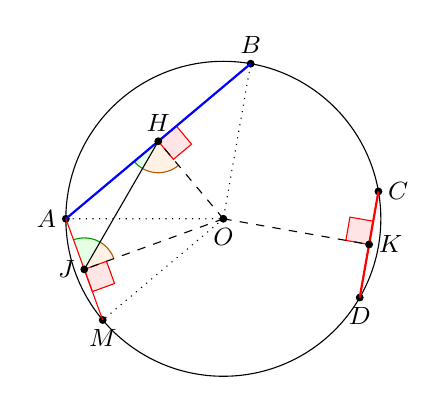
\begin{tikzpicture}[scale=1,font=\small]
\usetikzlibrary{calc}

\begin{scope}
\pgfmathsetmacro{\aalpha}{-20};
\pgfmathsetmacro{\abeta}{40};
\pgfmathsetmacro{\agamma}{(\abeta+\aalpha)/2};

\coordinate (o) at (0,0);

\draw (o) circle (2);
\draw[fill] (o) circle (1.2pt) node[below] {$O$};

\path (o) -- (80:2) coordinate (b);
\path (o) -- (180:2) coordinate (a);
\path (o) -- (130:2) coordinate (o1);
\coordinate (h) at (intersection of o--o1 and a--b);

\path (o) -- (10:2) coordinate (c);
\path (o) -- (-30:2) coordinate (d);
\path (o) -- (-10:2) coordinate (o2);
\coordinate (k) at (intersection of o--o2 and c--d);

\path (o) -- (220:2) coordinate (m);
\path (o) -- (200:2) coordinate (o3);
\coordinate (j) at (intersection of o--o3 and a--m);

\begin{scope}
\clip (o) -- (j) -- (h) -- cycle;
\draw[orange!70!black, fill=orange!10] (h) circle (0.4);
\draw[orange!70!black, fill=orange!10] (j) circle (0.4);
\end{scope}

\begin{scope}
\clip (a) -- (j) -- (h) -- cycle;
\draw[green!60!black, fill=green!10] (h) circle (0.4);
\draw[green!60!black, fill=green!10] (j) circle (0.4);
\end{scope}

\draw[dotted] (a) -- (o) -- (b);
\draw[dotted] (o) -- (m);

\draw[fill] (a) circle (1.2pt) node[left] {$A$};
\draw[fill] (b) circle (1.2pt) node[above] {$B$};
\begin{scope}[rotate=40]
\draw[red,fill=red!10] (h) rectangle ([shift={(0.3,-0.3)}]h);
\end{scope}
\draw[thick, blue] (a) -- (b);
\draw[fill] (h) circle (1.2pt) node[above] {$H$};
\draw[dashed] (o) -- (h);

\draw[fill] (c) circle (1.2pt) node[right] {$C$};
\draw[fill] (d) circle (1.2pt) node[below] {$D$};
\begin{scope}[rotate=-10]
\draw[red,fill=red!10] (k) rectangle ([shift={(-0.3,0.3)}]k);
\end{scope}
\draw[thick, red] (c) -- (d);
\draw[fill] (k) circle (1.2pt) node[right] {$K$};
\draw[dashed] (o) -- (k);

\draw[fill] (m) circle (1.2pt) node[below] {$M$};
\begin{scope}[rotate=200]
\draw[red,fill=red!10] (j) rectangle ([shift={(-0.3,0.3)}]j);
\end{scope}
\draw[red] (a) -- (m);
\draw[fill] (j) circle (1.2pt) node[left] {$J$};
\draw[dashed] (o) -- (j);

\draw (h) -- (j);


\end{scope}

\end{tikzpicture}

\end{minipage}\vspace{10pt}

\noindent Viceversa\vspace{10pt}

\noindent Ipotesi:
\begin{itemize*}
\item $OH<OK$ (distanze disuguali),
\item $OH\perp AB$ ($OH$ distanza della corda $AB$ dal centro $O$),
\item $OK\perp CD$ ($OK$ distanza della corda $CD$ dal centro $O$).
\end{itemize*}
\noindent Tesi: $AB>CD$.

\begin{proof}
Utilizziamo un metodo simile alla dimostrazione per assurdo, come abbiamo già fatto per la dimostrazione delle disuguaglianze tra gli elementi di un triangolo: esaminiamo tutti i casi possibili ed escludiamo i casi che contraddicono il teorema precedente ed il primo caso di questo teorema.
Sono possibili le seguenti relazioni tra le lunghezze delle corde $AB$ e $CD$:
\[\text{(1) }AB\cong CD\text{;}\qquad\qquad\text{(2) }AB < CD\text{;}\qquad\qquad\text{(3) }AB > CD\text{.}\]

Se fosse vera la relazione (1), per il teorema precedente risulterebbe $OH\cong OK$, contro l'ipotesi.

Se fosse vera la (2), per la prima parte di questo stesso teorema risulterebbe $OH > OK$, contro l'ipotesi.

Rimane solo la possibilità che valga la relazione (3), la quale non è in contraddizione con la prima parte del teorema e che anzi la conferma. Dunque la tesi è verificata.
\end{proof}

Osservazioni:
\begin{itemize*}
\item Fissato un punto $P$, per esso passano infinite circonferenze.

Infatti, si consideri un qualunque altro punto $Q$: quest'ultimo può essere il centro di una circonferenza di raggio $QP$.

\item Per due punti fissati $A$ e $B$ passano infinite circonferenze.

Infatti, poiché tutti i punti dell'asse del segmento $AB$ sono equidistanti sia da $A$ che da $B$, essi possono essere centri di circonferenze passanti sia per $A$ che per $B$.
\end{itemize*}

\begin{definizione}
L'insieme di tutte le circonferenze passanti per due punti $A$ e $B$ è detto \emph{fascio di circonferenze}. Chiamiamo $A$ e $B$ \emph{punti base del fascio}, la retta per $A$ e $B$ \emph{asse radicale} e \emph{asse centrale} l'asse del segmento $AB$ che contiene tutti i centri delle circonferenze del fascio.
\end{definizione}

\begin{teorema}
Per tre punti distinti non allineati passa una ed una sola circonferenza.
\end{teorema}

\noindent\begin{minipage}{0.65\textwidth}\parindent15pt
\begin{proof}
Siano $A$, $B$ e $C$ tre punti non allineati e congiungiamo $A$ con $B$ e $B$ con $C$. Allora gli assi dei segmenti $AB$ e $BC$ si intersecheranno in un punto $O$. Per la proprietà degli assi il punto $O$, appartenendo a entrambi gli assi, è equidistante dai punti $A$, $B$ e $C$. Allora si può costruire una circonferenza con centro in $O$ e raggio $OA$. Questa circonferenza passa per $A$, $B$ e $C$, inoltre è unica perché è unico l'asse di un segmento e di conseguenza è unico il punto di intersezione tra i due assi.
\end{proof}
\end{minipage}\hfil
\begin{minipage}{0.35\textwidth}
	\centering% Copyright (c) 2015 Daniele Masini - d.masini.it@gmail.com

\begin{tikzpicture}[scale=.9,font=\small]
\usetikzlibrary{calc}

\begin{scope}
\pgfmathsetmacro{\aalpha}{-20};
\pgfmathsetmacro{\abeta}{40};
\pgfmathsetmacro{\agamma}{(\abeta+\aalpha)/2};

\coordinate (o) at (0,0);

\draw[dotted] (o) circle (2);
\draw[fill] (o) circle (1.2pt) node[right] {$O$};

\path (o) -- (80:2) coordinate (b);
\path (o) -- (140:2) coordinate (a);
\path (o) -- (110:2) coordinate (o1);
\coordinate (h) at (intersection of o--o1 and a--b);

\path (o) -- (10:2) coordinate (c);
\path (o) -- (45:2) coordinate (o2);
\coordinate (k) at (intersection of o--o2 and b--c);

\draw[fill] (a) circle (1.2pt) node[left] {$A$};
\draw[fill] (b) circle (1.2pt) node[above] {$B$};
\draw (a) -- (b);
%\draw[fill] (h) circle (1.2pt) node[above] {$H$};
\draw[dashdotted] ($(o)!-.5!(h)$) -- ($(o)!1.35!(h)$);

\draw[fill] (c) circle (1.2pt) node[right] {$C$};
\draw (b) -- (c);
%\draw[fill] (k) circle (1.2pt) node[right] {$K$};
\draw[dashdotted] ($(o)!-.5!(k)$) -- ($(o)!1.5!(k)$);

\end{scope}

\end{tikzpicture}

\end{minipage}

\osservazione
L'ipotesi che i punti siano non allineati è essenziale. Seguendo le linee della dimostrazione, i segmenti $AB$ e $BC$ sono consecutivi ma non adiacenti, cosa essenziale per affermare che i rispettivi assi non sono paralleli. Vale infatti anche la seguente proprietà:
\begin{teorema}
Dati tre punti distinti $A$, $B$ e $C$ appartenenti ad una stessa retta, non esiste alcuna circonferenza che passa per $A$, $B$ e $C$.
\end{teorema}

\begin{figure}[htb]
	\centering% Copyright (c) 2015 Daniele Masini - d.masini.it@gmail.com

\begin{tikzpicture}[scale=1,font=\small]
\usetikzlibrary{calc}

\begin{scope}

\draw (0,0) coordinate (a) -- (1,0) coordinate (b) -- (3,0) coordinate (c);

\draw[fill] (a) circle (1.2pt) node[above] {$A$};
\draw[fill] (b) circle (1.2pt) node[above] {$B$};
\draw[fill] (c) circle (1.2pt) node[above] {$C$};
\draw[dashdotted] (0.5,0.5) -- (0.5,-1.5);
\draw[dashdotted] (2,0.5) -- (2,-1.5);

\end{scope}

\end{tikzpicture}

\end{figure}

\begin{proof}
Verifichiamo che non esiste alcun punto del piano individuato da $A$, $B$ e $C$ che possa essere il centro di una tale circonferenza, cioè che sia equidistante dai tre punti.
Supponendo per assurdo che esista un tal punto $O$, questo, dovendo essere equidistante da $A$ e da $B$, dovrebbe appartenere all'asse del segmento $AB$ (luogo dei punti equidistanti dagli estremi) e, per ragioni analoghe, dovrebbe appartenere anche all'asse del segmento $BC$. Ma i punti $A$, $B$ e $C$ sono distinti per ipotesi, in particolare $A$ e $C$ non sono sovrapposti. Quindi, detto $M$ il punto medio di $AB$ ed $N$ il punto medio di $BC$, $M$ ed $N$ sono anch'essi distinti e pertanto gli assi dei segmenti $AB$, $BC$ non possono essere coincidenti; inoltre gli assi dei segmenti $AB$, $BC$ sono entrambi perpendicolari alla stessa retta che contiene i tre punti $A$, $B$, $C$ e quindi sono paralleli tra loro; essendo dunque rette parallele e distinte, i due assi non hanno punti in comune e pertanto non può esistere un punto $O$ che possa essere il centro della circonferenza passante per $A$, $B$ e $C$.
\end{proof}

\begin{corollario}
Tre punti qualsiasi appartenenti ad una circonferenza non sono allineati.
\end{corollario}

A conclusione di queste prime proprietà, possiamo enunciare il seguente
\begin{corollario}
Una circonferenza è univocamente determinata dal suo centro e dal suo raggio oppure da tre suoi punti.
\end{corollario}

Diamo ora la definizione di alcune parti del cerchio e della circonferenza. Ne esamineremo le proprietà in seguito.
\begin{definizione}
Data una circonferenza di centro $O$,
\begin{itemize*}
\item chiamiamo \emph{angolo al centro} un qualunque angolo con vertice in $O$;
\item l'intersezione della circonferenza con un angolo al centro $\gamma$ è detta \emph{arco} e diremo che l'angolo $\gamma$ insiste su tale arco;
\item i punti di intersezione della circonferenza con i lati dell'angolo si dicono \emph{estremi dell'arco};
\item un arco individuato da un angolo al centro piatto si chiama \emph{semicirconferenza}.
\end{itemize*}
\end{definizione}

\noindent\begin{minipage}{0.6\textwidth}\parindent15pt
Ogni coppia di punti distinti su una circonferenza individua due archi sulla medesima circonferenza. Infatti se consideriamo $A$ e $B$ ottenuti come nella definizione precedente questi punti individuano l'arco su cui insiste l'angolo $\gamma$ ma anche la restante parte di circonferenza che è pure un arco.
Congiungendo $A$ con $B$ il segmento $AB$ è una corda della circonferenza. Diremo che la corda $AB$ sottende l'arco $AB$ o viceversa che l'arco insiste sulla corda.
Se in particolare i punti $A$ e $B$ sono diametralmente opposti, essi individuano sulla circonferenza due archi che sono due semicirconferenze.
\end{minipage}\hfil
\begin{minipage}{0.4\textwidth}
	\centering% Copyright (c) 2015 Daniele Masini - d.masini.it@gmail.com

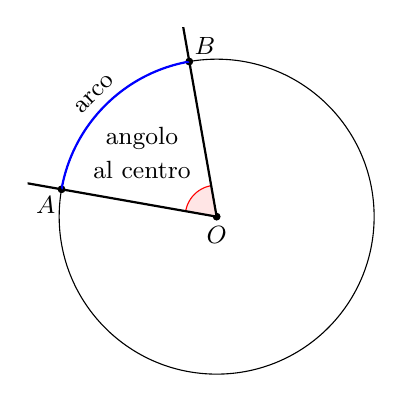
\begin{tikzpicture}[scale=1,font=\small]
\usetikzlibrary{calc}

\begin{scope}
\clip (-2.4,-2.01) rectangle (2.1,2.4);
\coordinate (o) at (0,0);

\draw (o) circle (2);
\draw[fill] (o) circle (1.2pt) node[below] {$O$};

\path (o) -- (100:2) coordinate (b);
\path (o) -- (170:2) coordinate (a);

\begin{scope}
\clip (a) -- (o) -- (b) -- cycle;
\draw[red, fill=red!10] (o) circle (0.4);
\end{scope}

\draw[thick] ($(a)!-.25!(o)$) -- (o) -- ($(b)!-.25!(o)$);

\draw[fill] (a) circle (1.2pt) node[shift={(-0.2,.-0.2)}] {$A$};
\draw[fill] (b) circle (1.2pt) node[shift={(0.2,0.2)}] {$B$};

\begin{scope}
\clip (a) -- (o) -- ++(b) -- ++($(a)-(o)$) -- cycle;
\draw[thick, blue] (o) circle (2) node[black, shift={(135:2.2)}, rotate=45] {arco};
\node at (-0.95,1) {angolo};
\node at (-0.95,0.6) {al centro};
\end{scope}

\end{scope}

\end{tikzpicture}

\end{minipage}

\begin{definizione}Dato un cerchio
\begin{itemize*}
\item si dice \emph{settore circolare} l'intersezione del cerchio con un suo angolo al centro: se l'angolo al centro è piatto di parla di \emph{semicerchio};
\item si chiama \emph{segmento circolare ad una base} la parte di cerchio limitata da una corda e da un arco che vi insiste; la corda viene detta \emph{base del segmento circolare};
\item la parte di cerchio limitata da due corde parallele è detta \emph{segmento circolare a due basi}, le due corde prendono il nome di \emph{basi del segmento circolare} e la loro distanza si dice \emph{altezza del segmento circolare}.
\end{itemize*}
\end{definizione}

Ogni corda divide il cerchio in due segmenti circolari ad una base. In particolare se la corda è un diametro otteniamo due semicerchi.
Un semicerchio, quindi, è sia un particolare settore circolare sia un particolare segmento circolare. \`E anche l'unico caso possibile di settore che sia anche segmento o viceversa.

\noindent\begin{minipage}{0.5\textwidth}\parindent15pt
Una coppia di corde parallele individua in un cerchio un segmento circolare a due basi e due segmenti circolari ad una base (se vogliamo considerare solo le tre parti non sovrapposte che hanno in comune al massimo una corda). Più in generale, date due corde parallele e distinte, queste individuano un segmento circolare a due basi e quattro segmenti circolari ad una base, ed il segmento a due basi è anche l'intersezione dei due segmenti ad una base ``sovrapposti''.
\end{minipage}\hfil
\begin{minipage}{0.5\textwidth}
	\centering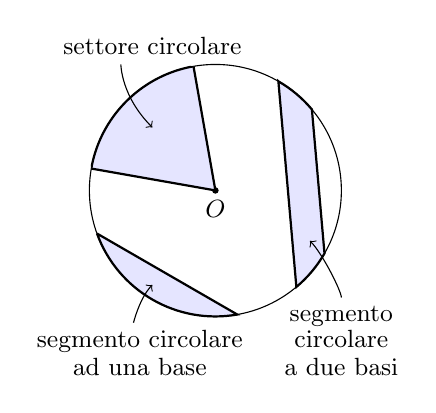
\begin{tikzpicture}[scale=.8,font=\small]
\usetikzlibrary{calc}

\begin{scope}
%\clip (-2.01,-2.01) rectangle (2.01,2.01);
\coordinate (o) at (0,0);

\draw (o) circle (2);
\draw[fill] (o) circle (1.2pt) node[below] {$O$};

\coordinate (a) at (170:2);
\coordinate (b) at (100:2);
\coordinate (c) at (200:2);
\coordinate (d) at (280:2);

\coordinate (e) at (60:2);
\coordinate (f) at (40:2);
\coordinate (g) at (-50:2);
\coordinate (h) at (-30:2);

\begin{scope}
\clip (a) -- (o) -- ++(b) -- ++($(a)-(o)$) -- cycle;
\draw[thick, fill=blue!10] (o) circle (2);
\end{scope}

\draw[thick] (a) -- (o) -- (b);
\draw[thick, fill=blue!10] (c) -- (d) arc (280:200:2) -- cycle;
\draw[thick, fill=blue!10] (e) -- (g) arc (-50:-30:2) -- (h) -- (f) arc (40:60:2) -- cycle;

\coordinate (setc) at (-1,1);
\coordinate (setc_d) at (-1,2.3);
\node at (setc_d) {settore circolare};
\draw[->] ([shift={(-.5,-.3)}]setc_d) .. controls ([shift={(-.5,-.3)}]setc_d) and ([shift={(-.5,.5)}]setc) .. (setc);

\coordinate (segc) at (-1,-1.5);
\coordinate (segc_d) at (-1.2,-2.4);
\node at (segc_d) {segmento circolare};
\node at ([shift={(0,-.4)}]segc_d) {ad una base};
\draw[->] ([shift={(-.1,.3)}]segc_d) .. controls ([shift={(-.1,.3)}]segc_d) and ([shift={(-.2,-.2)}]segc) .. (segc);

\coordinate (segcc) at (1.5,-.8);
\coordinate (segcc_d) at (2,-2);
\node at (segcc_d) {segmento};
\node at ([shift={(0,-.36)}]segcc_d) {circolare};
\node at ([shift={(0,-.8)}]segcc_d) {a due basi};
\draw[->] ([shift={(0,.3)}]segcc_d) .. controls ([shift={(0,.4)}]segcc_d) and ([shift={(.2,-.2)}]segcc) .. (segcc);



\end{scope}

\end{tikzpicture}

\end{minipage}

\section{Posizioni relative fra rette e circonferenze}

Perché alcune strade a scorrimento veloce vengono chiamate ``tangenziali''?
Per rispondere a questa domanda dobbiamo definire le posizioni che può assumere una retta rispetto ad una circonferenza.
Consideriamo in uno stesso piano una circonferenza $C$ di centro $O$ e raggio $r$ e una retta generica $m$; la distanza $d$ fra il centro $O$ e la retta $m$ è definita dal segmento $OH$, che ha un estremo coincidente con il centro $O$ ed è perpendicolare in $H$ alla retta $m$ ($H$ è il piede della perpendicolare). Si possono distinguere i tre casi seguenti:\vspace{4pt}

\begin{enumeratea}

\noindent\begin{minipage}{0.6\textwidth}\parindent15pt
\item $d > r$ : la distanza del centro $O$ dalla retta è maggiore del raggio.\\
Il punto $H$ è esterno alla circonferenza così come ogni altro punto della retta $m$. La retta si dice allora \emph{esterna} alla circonferenza e non ha alcun punto in comune con essa, ovvero non vi sono punti di intersezione fra $C$ ed $m$.
\end{minipage}\hfil
\begin{minipage}{0.4\textwidth}
	\centering% Copyright (c) 2015 Daniele Masini - d.masini.it@gmail.com

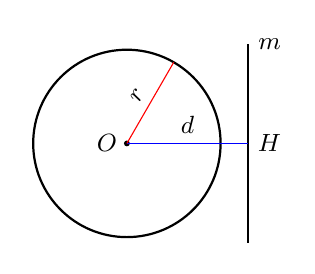
\begin{tikzpicture}[scale=.7,font=\small]
\usetikzlibrary{calc}

\begin{scope}
\pgfmathsetmacro{\raggio}{1.7}
\clip (-\raggio-0.1,-\raggio-0.15) rectangle (2.9,\raggio+.4);
\coordinate (o) at (0,0);

\draw[thick] (o) circle (\raggio);
\draw[fill] (o) circle (1.2pt) node[left] {$O$};

\coordinate (r1) at (2.2,1.8);
\coordinate (r2) at (2.2,-1.8);

\coordinate (r) at (60:\raggio);

\draw[thick] (r1) node[right] {$m$} -- (r2);
\draw[blue] (o) -- node[black, above, midway, sloped] {$d$} ($(r1)!(o)!(r2)$) node[black, right] {$H$};
\draw[red] (o) -- node[black, above, midway, sloped] {$r$} (r);

\end{scope}

\end{tikzpicture}
\\\vspace{5pt}
\end{minipage}\vspace{4pt}

\noindent\begin{minipage}{0.6\textwidth}\parindent15pt
\item $d < r$ : la distanza del centro $O$ dalla retta è minore del raggio.\\
La retta $m$ interseca la circonferenza in due punti distinti $A$ e $B$; questi appartengono alla circonferenza e quindi $OA\cong OB\cong r$. Il segmento $AB$ appartiene alla retta e definisce anche la corda $AB$, i cui punti, tutti interni alla circonferenza, hanno una distanza dal centro minore del raggio; il punto di minore distanza è proprio $H$, che è anche il punto medio della corda $AB$. I punti della retta non appartenenti alla corda $AB$ sono esterni alla circonferenza e la loro distanza dal centro $O$ è maggiore del raggio.
La retta viene detta \emph{secante} alla circonferenza nei punti $A$ e $B$, che sono i punti di intersezione della retta con la circonferenza stessa.
\end{minipage}\hfil
\begin{minipage}{0.4\textwidth}
	\centering% (c) 2014 Daniele Masini - d.masini.it@gmail.com
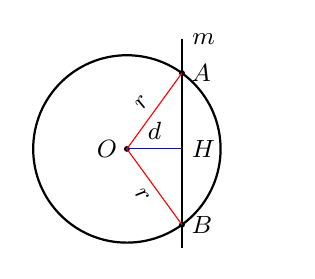
\begin{tikzpicture}[scale=.7,font=\small]
\usetikzlibrary{calc,intersections}

\begin{scope}
\pgfmathsetmacro{\raggio}{1.7}
\clip (-\raggio-0.1,-\raggio-0.15) rectangle (2.9,\raggio+.5);
\coordinate (o) at (0,0);

\draw[name path=Circle1, thick] (o) circle (\raggio);
\draw[fill] (o) circle (1.2pt) node[left] {$O$};

\coordinate (r1) at (1,2);
\coordinate (r2) at (1,-1.8);

\draw[name path=Retta, thick] (r1) -- (r2);

\draw[thick] (r1) node[right] {$m$} -- (r2);
\draw[blue] (o) -- node[black, above, midway, sloped] {$d$} ($(r1)!(o)!(r2)$) node[black, right] {$H$};

\path [name intersections={of=Circle1 and Retta}] ;
\draw[fill] (intersection-1) coordinate (a) circle (1.2pt) node[right] {$A$};
\draw[fill] (intersection-2) coordinate (b) circle (1.2pt) node[right] {$B$};
\draw[red] (a) -- node[black, above, midway, sloped] {$r$} (o) -- node[black, below, midway, sloped] {$r$} (b);

\end{scope}

\end{tikzpicture}
\\\vspace{4pt}
	\centering% Copyright (c) 2015 Daniele Masini - d.masini.it@gmail.com

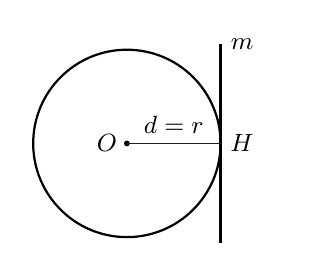
\begin{tikzpicture}[scale=.7,font=\small]
\usetikzlibrary{calc,intersections}

\begin{scope}
\pgfmathsetmacro{\raggio}{1.7}
\clip (-\raggio-0.1,-\raggio-0.15) rectangle (2.9,\raggio+.4);
\coordinate (o) at (0,0);

\draw[name path=Circle1, thick] (o) circle (\raggio);
\draw[fill] (o) circle (1.2pt) node[left] {$O$};

\coordinate (r1) at (\raggio,1.8);
\coordinate (r2) at (\raggio,-1.8);

\draw[name path=Retta, thick] (r1) -- (r2);

\draw[thick] (r1) node[right] {$m$} -- (r2);
\draw[blue] (o) -- node[black, above, midway, sloped] {$d=r$} ($(r1)!(o)!(r2)$) node[black, right] {$H$};

\end{scope}

\end{tikzpicture}
\\\vspace{4pt}
\end{minipage}\vspace{4pt}

\item $d = r$ : la distanza del centro $O$ dalla retta è pari al raggio.\\
Il punto $H$ appartiene alla circonferenza mentre ogni altro punto della retta $m$ è esterno alla circonferenza e ha una distanza dal centro $O$ maggiore del raggio. La retta viene detta \emph{tangente} alla circonferenza e $H$ è il punto di tangenza o di contatto.

\end{enumeratea}

\noindent\begin{minipage}{0.5\textwidth}\parindent15pt
Si noti che la retta tangente è perpendicolare al raggio nel punto di tangenza. Inoltre, l'unica retta perpendicolare al raggio nel punto di intersezione tra il raggio e la circonferenza è tangente.
Consideriamo una circonferenza $C$ di centro $O$ e raggio $r$ e una retta $m$ ad essa secante nei punti distinti $A$ e $B$. Sia $OH$ la distanza del centro $O$ dalla retta. 
Trasliamo la retta $m$ in modo da aumentare la sua distanza dal centro $O$ (vedi figura). All'aumentare della distanza $d = OH$, quella fra i punti $A$ e $B$ diminuisce; quando $OH = r$, i punti $A$ e $B$ coincidono nel punto di tangenza. Dunque la tangente è un caso particolare di secante avente due punti di intersezione coincidenti.
\end{minipage}\hfil
\begin{minipage}{0.5\textwidth}
	\centering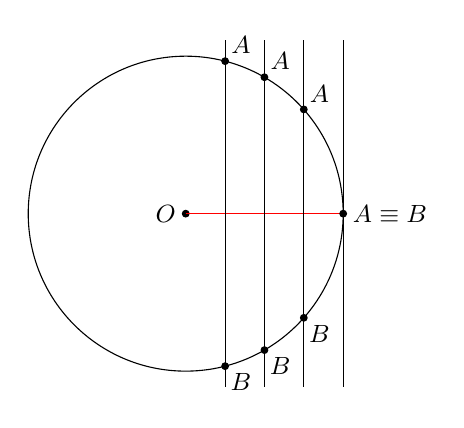
\begin{tikzpicture}[scale=1,font=\small]
\usetikzlibrary{calc,intersections}

\begin{scope}
\pgfmathsetmacro{\raggio}{2}
\coordinate (o) at (0,0);

\draw[name path=Circle1] (o) circle (\raggio);
\draw[fill] (o) circle (1.2pt) node[left] {$O$};

\draw[red] (o) -- (\raggio,0);

\coordinate (r11) at (0.5,2.2);
\coordinate (r12) at (0.5,-2.2);
\draw[name path=Retta1] (r11) -- (r12);
\path [name intersections={of=Circle1 and Retta1}] ;
\draw[fill] (intersection-1) coordinate (a1) circle (1.2pt) node[shift={(.2,.2)}] {$A$};
\draw[fill] (intersection-2) coordinate (b1) circle (1.2pt) node[shift={(.2,-.2)}] {$B$};

\coordinate (r21) at (1,2.2);
\coordinate (r22) at (1,-2.2);
\draw[name path=Retta2] (r21) -- (r22);
\path [name intersections={of=Circle1 and Retta2}] ;
\draw[fill] (intersection-1) coordinate (a2) circle (1.2pt) node[shift={(.2,.2)}] {$A$};
\draw[fill] (intersection-2) coordinate (b2) circle (1.2pt) node[shift={(.2,-.2)}] {$B$};

\coordinate (r31) at (1.5,2.2);
\coordinate (r32) at (1.5,-2.2);
\draw[name path=Retta3] (r31) -- (r32);
\path [name intersections={of=Circle1 and Retta3}] ;
\draw[fill] (intersection-1) coordinate (a3) circle (1.2pt) node[shift={(.2,.2)}] {$A$};
\draw[fill] (intersection-2) coordinate (b3) circle (1.2pt) node[shift={(.2,-.2)}] {$B$};

\coordinate (r41) at (2,2.2);
\coordinate (r42) at (2,-2.2);
\draw[name path=Retta4] (r41) -- (r42);
\draw[fill] (2,0) coordinate (a4) circle (1.2pt) node[right] {$A\equiv B$};

\end{scope}

\end{tikzpicture}

\end{minipage}

\noindent\begin{minipage}{0.5\textwidth}\parindent15pt
Una più efficace ``visualizzazione'' di questo concetto è la seguente.
Consideriamo la stessa circonferenza e la stessa retta dell'esempio precedente. Ruotiamo la retta attorno al punto $B$ (vedi figura).
La distanza del punto $A$ dal punto $B$ diminuisce all'aumentare dell'angolo $O\widehat{B}A$ fra la retta e il raggio. Quando il punto $A$ coincide con il punto $B$, il raggio è perpendicolare alla retta e quest'ultima è tangente alla circonferenza in $B\equiv A$.
\end{minipage}\hfil
\begin{minipage}{0.5\textwidth}
	\centering% (c) 2014 Daniele Masini - d.masini.it@gmail.com
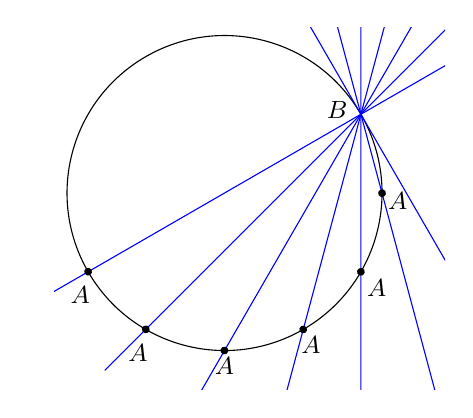
\begin{tikzpicture}[scale=1,font=\small]
\usetikzlibrary{calc,intersections}

\clip (-2.5, -2.5) rectangle (2.8,2.1);

\begin{scope}[rotate=30]
\pgfmathsetmacro{\raggio}{2}

\coordinate (o) at (0,0);

\draw[name path=Circle1] (o) circle (\raggio);
%\draw[fill] (o) circle (1.2pt) node[left] {$O$};

\coordinate (b) at (\raggio,0);
\draw [blue,name path=Retta1] (b) node[black,shift={(-.3,.05)}] {$B$} -- +(0:-4.5) -- +(0:4.2);
\path [name intersections={of=Circle1 and Retta1}] ;
\draw[fill] (intersection-2) coordinate (a1) circle (1.2pt) node[shift={(-.1,-.3)}] {$A$};
%\draw[fill] (intersection-2) coordinate (b1) circle (1.2pt) node[shift={(.2,-.2)}] {$B$};

\draw [blue,name path=Retta2] (b) -- +(15:-4.6) -- +(15:4.2);
\path [name intersections={of=Circle1 and Retta2}] ;
\draw[fill] (intersection-2) coordinate (a1) circle (1.2pt) node[shift={(-.1,-.3)}] {$A$};

\draw [blue,name path=Retta3] (b) -- +(30:-4.2) -- +(30:4.2);
\path [name intersections={of=Circle1 and Retta3}] ;
\draw[fill] (intersection-2) coordinate (a1) circle (1.2pt) node[shift={(0,-.2)}] {$A$};

\draw [blue,name path=Retta4] (b) -- +(45:-4.2) -- +(45:4.2);
\path [name intersections={of=Circle1 and Retta4}] ;
\draw[fill] (intersection-2) coordinate (a1) circle (1.2pt) node[shift={(.1,-.2)}] {$A$};

\draw [blue,name path=Retta5] (b) -- +(60:-4.2) -- +(60:4.2);
\path [name intersections={of=Circle1 and Retta5}] ;
\draw[fill] (intersection-1) coordinate (a1) circle (1.2pt) node[shift={(.2,-.2)}] {$A$};

\draw [blue,name path=Retta6] (b) -- +(75:-4.2) -- +(75:4.2);
\path [name intersections={of=Circle1 and Retta6}] ;
\draw[fill] (intersection-2) coordinate (a1) circle (1.2pt) node[shift={(.2,-.1)}] {$A$};

\draw [blue,name path=Retta7] (b) -- +(90:-4.2) -- +(90:4.2);

\end{scope}

\end{tikzpicture}

\end{minipage}

Il lettore dimostri per esercizio il seguente teorema (si suggerisce di ricorrere alla dimostrazione per assurdo).
\begin{teorema}
Se una retta è esterna ad una circonferenza, allora la sua distanza dal centro è maggiore del raggio, se è tangente la distanza dal centro è uguale al raggio e se è secante la distanza dal centro è minore del raggio.
\end{teorema}

Possiamo ora rispondere al quesito iniziale. Il termine ``tangenziale'' viene utilizzato per descrivere una strada a scorrimento veloce, realizzata in zone particolarmente urbanizzate, per permettere il transito degli autoveicoli senza dover entrare in contatto diretto con la circolazione urbana; ciò comporta evidenti benefici per la vivibilità dei centri cittadini. Possiamo immaginare il centro città racchiuso in un cerchio e la tangenziale come una retta di un certo spessore che è, appunto, tangente al cerchio.

\subsection{Posizioni reciproche di due circonferenze}

Descriviamo adesso le posizioni reciproche di due circonferenze.
\begin{definizione}
Due circonferenze si dicono:
\begin{itemize*}
\item \emph{esterne} se tutti i punti dell'una sono esterni all'altra;
\item \emph{secanti} quando hanno due punti in comune;
\item \emph{una interna all'altra} se i loro raggi sono diseguali e i punti della circonferenza di raggio minore sono tutti interni a quella di raggio maggiore;
\item \emph{tangenti} se hanno un solo punto in comune detto punto di tangenza; si possono inoltre distinguere fra: 
\begin{itemize*}
\item \emph{tangenti esternamente} se, ad eccezione del punto di tangenza, tutti i punti di una circonferenza sono esterni all'altra;
\item \emph{tangenti internamente} se i loro raggi sono diseguali e, ad eccezione del punto di tangenza, tutti i punti della circonferenza di raggio minore sono interni a quella di raggio maggiore.
\end{itemize*}
\end{itemize*}
\end{definizione}

Analizziamo in dettaglio i diversi casi; come esercizio lasciamo allo studente la dimostrazione rigorosa delle seguenti proprietà.

\begin{teorema}
Date due circonferenze esterne, la distanza fra i due centri è maggiore della somma dei raggi.
\end{teorema}

\begin{figure}[htb]
	\centering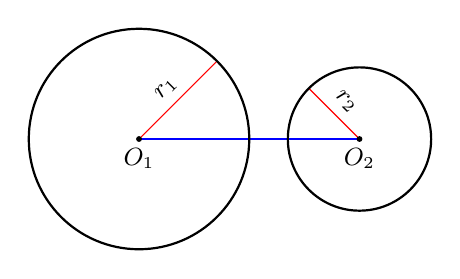
\begin{tikzpicture}[scale=.7,font=\small]
\usetikzlibrary{calc,intersections}

\begin{scope}
\pgfmathsetmacro{\raggioa}{2}
\pgfmathsetmacro{\raggiob}{1.3}
\coordinate (oa) at (0,0);
\coordinate (ob) at (4,0);

\draw[blue] (oa) -- (ob);

\draw[red] (oa) -- node[black, above, midway, sloped] {$r_1$} (45:\raggioa);
\draw[thick, name path=Circle1] (oa) circle (\raggioa);
\draw[fill] (oa) circle (1.2pt) node[below] {$O_1$};

\draw[red] (ob) -- node[black, above, midway, sloped] {$r_2$} +(135:\raggiob);
\draw[thick, name path=Circle2] (ob) circle (\raggiob);
\draw[fill] (ob) circle (1.2pt) node[below] {$O_2$};


\end{scope}

\end{tikzpicture}

\end{figure}

Abbiamo già dimostrato che per tre punti distinti non allineati passa una sola circonferenza, mentre per due punti passano infinite circonferenze. Di conseguenza due circonferenze distinte possono avere al massimo due punti in comune. \`E il caso delle circonferenze secanti. Se invece il numero di punti in comune è uno, allora ci riduciamo al caso delle circonferenze tangenti.

\begin{teorema}
Date due circonferenze secanti, la distanza fra i centri è maggiore della differenza dei raggi e minore della loro somma.
\end{teorema}

\begin{figure}[htb]
	\centering% Copyright (c) 2015 Daniele Masini - d.masini.it@gmail.com

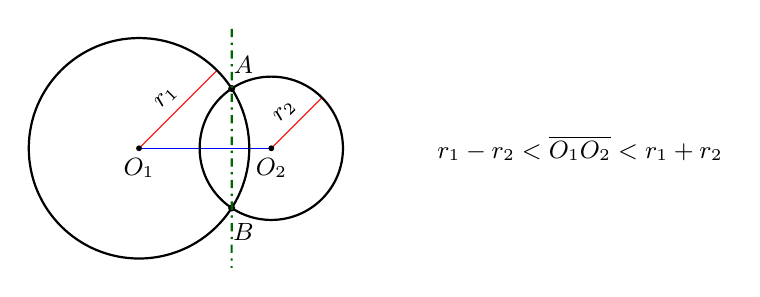
\begin{tikzpicture}[scale=.7,font=\small]
\usetikzlibrary{calc,intersections}

\begin{scope}
\pgfmathsetmacro{\raggioa}{2}
\pgfmathsetmacro{\raggiob}{1.3}
\coordinate (oa) at (0,0);
\coordinate (ob) at (2.4,0);

\draw[blue] (oa) -- (ob);

\draw[red] (oa) -- node[black, above, midway, sloped] {$r_1$} (45:\raggioa);
\draw[thick, name path=Circle1] (oa) circle (\raggioa);
\draw[fill] (oa) circle (1.2pt) node[below] {$O_1$};

\draw[red] (ob) -- node[black, above, midway, sloped] {$r_2$} +(45:\raggiob);
\draw[thick, name path=Circle2] (ob) circle (\raggiob);
\draw[fill] (ob) circle (1.2pt) node[below] {$O_2$};

\path [name intersections={of=Circle1 and Circle2}] ;
\draw[fill] (intersection-1) coordinate (a) circle (1.5pt) node[shift={(.15,.3)}] {$A$};
\draw[fill] (intersection-2) coordinate (b) circle (1.5pt) node[shift={(.15,-.3)}] {$B$};
\draw[thick,green!40!black,dashdotted] ($(a)!-0.5!(b)$)--($(a)!1.5!(b)$);

\node at (8,0) {$\abs{r_1-r_2}<\overline{O_1O_2}<r_1+r_2$};

\end{scope}

\end{tikzpicture}

\end{figure}

La retta passante per i punti di intersezione viene detta \emph{asse radicale}.

Si dimostra che l'asse radicale è perpendicolare alla retta congiungente i centri.

\begin{teorema}
Data una circonferenza interna ad un'altra, la distanza fra i centri è minore della differenza fra i raggi.
\end{teorema}

\begin{figure}[htb]
	\centering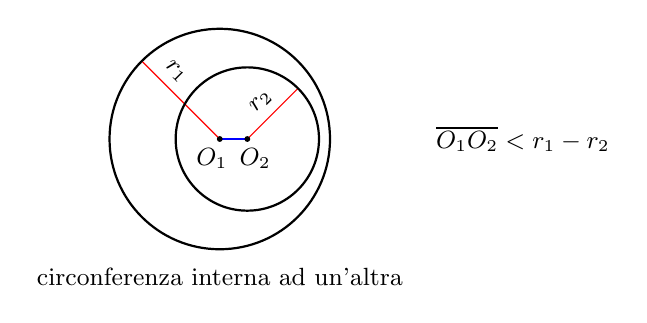
\begin{tikzpicture}[scale=.7,font=\small]
\usetikzlibrary{calc,intersections}

\begin{scope}
\pgfmathsetmacro{\raggioa}{2}
\pgfmathsetmacro{\raggiob}{1.3}
\coordinate (oa) at (0,0);
\coordinate (ob) at (.5,0);

\draw[blue] (oa) -- (ob);

\draw[red] (oa) -- node[black, above, midway, sloped, shift={(-.3,0)}] {$r_1$} (135:\raggioa);
\draw[thick, name path=Circle1] (oa) circle (\raggioa);
\draw[fill] (oa) circle (1.2pt) node[shift={(-.1,-.25)}] {$O_1$};

\draw[red] (ob) -- node[black, above, midway, sloped] {$r_2$} +(45:\raggiob);
\draw[thick, name path=Circle2] (ob) circle (\raggiob);
\draw[fill] (ob) circle (1.2pt) node[shift={(.1,-.25)}] {$O_2$};

\node at (0,-2.5) {circonferenza interna ad un'altra};

\node at (5.5,0) {$\overline{O_1O_2}<r_1-r_2$};

\end{scope}

\end{tikzpicture}
\hspace{1.5cm}% Copyright (c) 2015 Daniele Masini - d.masini.it@gmail.com

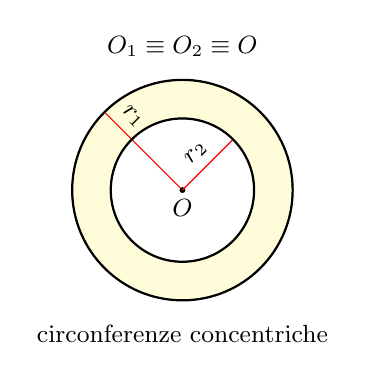
\begin{tikzpicture}[scale=.7,font=\small]
\usetikzlibrary{calc,intersections}

\begin{scope}
\pgfmathsetmacro{\raggioa}{2}
\pgfmathsetmacro{\raggiob}{1.3}
\coordinate (o) at (0,0);

\begin{scope}
\draw[fill=yellow!15] (o) circle (\raggioa);
\draw[fill=white] (o) circle (\raggiob);
\end{scope}


\draw[red] (o) -- node[black, above, midway, sloped, shift={(-0.4,0)}] {$r_1$} (135:\raggioa);
\draw[thick, name path=Circle1] (o) circle (\raggioa);
\draw[fill] (o) circle (1.2pt) node[below] {$O$};

\draw[red] (o) -- node[black, above, midway, sloped] {$r_2$} +(45:\raggiob);
\draw[thick, name path=Circle2] (o) circle (\raggiob);

\node at (0,2.6) {$O_1\equiv O_2\equiv O$};
\node at (0,-2.6) {circonferenze concentriche};

\end{scope}

\end{tikzpicture}

\end{figure}

Un caso particolare di circonferenze una interna all'altra è rappresentato dalle \emph{circonferenze concentriche}, i cui centri coincidono. La zona di piano delimitata dalle due circonferenze è detta \emph{corona circolare}.

\begin{teorema}
Date due circonferenze tangenti esternamente in un punto $T$, la distanza fra i centri è uguale alla somma dei raggi. La retta tangente passante per $T$ è comune alle due circonferenze ed è perpendicolare alla retta congiungente i due centri.
\end{teorema}

\begin{figure}[htb]
	\centering% (c) 2014 Daniele Masini - d.masini.it@gmail.com
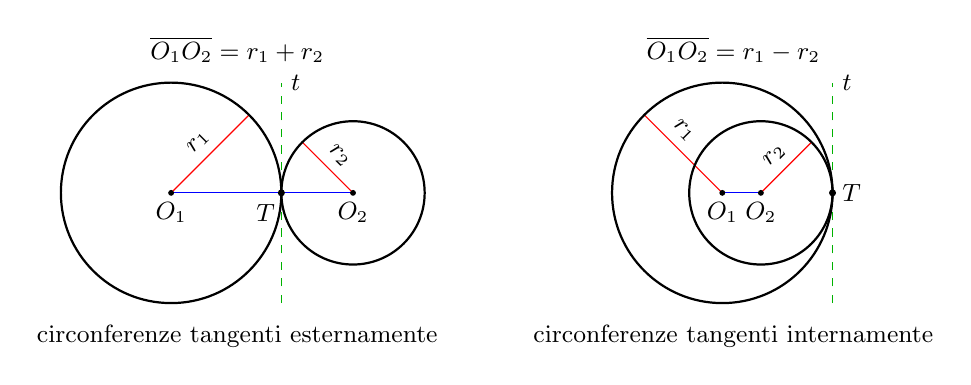
\begin{tikzpicture}[scale=.7,font=\small]
\usetikzlibrary{calc,intersections}

\begin{scope}
\pgfmathsetmacro{\raggioa}{2}
\pgfmathsetmacro{\raggiob}{1.3}
\coordinate (oa) at (0,0);
\coordinate (ob) at (3.3,0);

\draw[blue] (oa) -- (ob);
\draw[green!70!black, dashed] (2,-2) -- (2,2) node[black, right] {$t$};

\draw[red] (oa) -- node[black, above, midway, sloped] {$r_1$} (45:\raggioa);
\draw[thick, name path=Circle1] (oa) circle (\raggioa);
\draw[fill] (oa) circle (1.2pt) node[below] {$O_1$};

\draw[red] (ob) -- node[black, above, midway, sloped] {$r_2$} +(135:\raggiob);
\draw[thick, name path=Circle2] (ob) circle (\raggiob);
\draw[fill] (ob) circle (1.2pt) node[below] {$O_2$};

\draw[fill] (2,0) circle (1.5pt) node[shift={(-.2,-.25)}] {$T$};

\node at (1.2,2.6) {$\overline{O_1O_2}=r_1+r_2$};

\node at (1.2,-2.6) {circonferenze tangenti esternamente};

\end{scope}


\begin{scope}[xshift=10cm]
\pgfmathsetmacro{\raggioa}{2}
\pgfmathsetmacro{\raggiob}{1.3}
\coordinate (oa) at (0,0);
\coordinate (ob) at (0.7,0);

\draw[blue] (oa) -- (ob);
\draw[green!70!black, dashed] (2,-2) -- (2,2) node[black, right] {$t$};

\draw[red] (oa) -- node[black, above, midway, sloped, shift={(-.2,0)}] {$r_1$} (135:\raggioa);
\draw[thick, name path=Circle1] (oa) circle (\raggioa);
\draw[fill] (oa) circle (1.2pt) node[below] {$O_1$};

\draw[red] (ob) -- node[black, above, midway, sloped] {$r_2$} +(45:\raggiob);
\draw[thick, name path=Circle2] (ob) circle (\raggiob);
\draw[fill] (ob) circle (1.2pt) node[below] {$O_2$};

\draw[fill] (2,0) circle (1.5pt) node[right] {$T$};

\node at (0.2,2.6) {$\overline{O_1O_2}=\abs{r_1-r_2}$};

\node at (0.2,-2.6) {circonferenze tangenti internamente};

\end{scope}

\end{tikzpicture}

\end{figure}

\begin{teorema}
Date due circonferenze tangenti internamente, la distanza fra i centri è pari alla differenza dei raggi.
\end{teorema}


Anche per le circonferenze si può affermare che nel caso siano tangenti lo sono in due punti coincidenti; infatti se prendiamo due circonferenze secanti e man mano allontaniamo i loro centri, osserviamo che i due punti di intersezione si avvicinano sempre più fino a sovrapporsi nel momento in cui la distanza fra i loro centri è pari alla somma dei raggi.

\begin{figure}[htb]
	\centering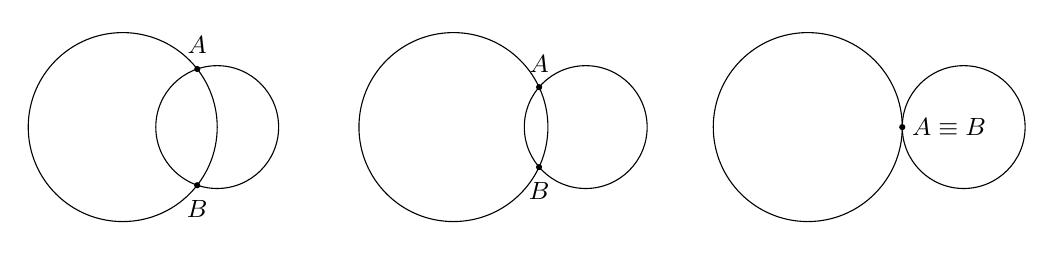
\begin{tikzpicture}[scale=.6,font=\small]
\usetikzlibrary{calc,intersections}

\begin{scope}
\pgfmathsetmacro{\raggioa}{2}
\pgfmathsetmacro{\raggiob}{1.3}
\coordinate (oa) at (0,0);
\coordinate (ob) at (2,0);

\draw[name path=Circle1] (oa) circle (\raggioa);
\draw[name path=Circle2] (ob) circle (\raggiob);

\path [name intersections={of=Circle1 and Circle2}] ;
\draw[fill] (intersection-1) coordinate (a) circle (1.5pt) node[shift={(0,.3)}] {$A$};
\draw[fill] (intersection-2) coordinate (b) circle (1.5pt) node[shift={(0,-.3)}] {$B$};

\end{scope}

\begin{scope}[xshift=7cm]
\pgfmathsetmacro{\raggioa}{2}
\pgfmathsetmacro{\raggiob}{1.3}
\coordinate (oa) at (0,0);
\coordinate (ob) at (2.8,0);

\draw[name path=Circle1] (oa) circle (\raggioa);
\draw[name path=Circle2] (ob) circle (\raggiob);

\path [name intersections={of=Circle1 and Circle2}] ;
\draw[fill] (intersection-1) coordinate (a) circle (1.5pt) node[shift={(0,.3)}] {$A$};
\draw[fill] (intersection-2) coordinate (b) circle (1.5pt) node[shift={(0,-.3)}] {$B$};

\end{scope}


\begin{scope}[xshift=14.5cm]
\pgfmathsetmacro{\raggioa}{2}
\pgfmathsetmacro{\raggiob}{1.3}
\coordinate (oa) at (0,0);
\coordinate (ob) at (3.3,0);

\draw[name path=Circle1] (oa) circle (\raggioa);
\draw[name path=Circle2] (ob) circle (\raggiob);

\draw[fill] (2,0) coordinate (a) circle (1.5pt) node[right] {$A\equiv B$};

\end{scope}


\end{tikzpicture}

\end{figure}

Se esaminiamo le varie posizioni reciproche nel caso di due circonferenze congruenti ($r_1 = r_2 = r$), tenendo conto anche del fatto banale che in tal caso $\abs{r_1 - r_2} = 0$ e $r_1 + r_2 = 2r$, scompaiono le ``distinte'' possibilità che esse siano concentriche, interne e tangenti internamente, ma compare la possibilità che siano coincidenti, cioè perfettamente sovrapposte.
Lasciamo al lettore la ``rivisitazione'' dei casi precedentemente analizzati nell'ipotesi che le due circonferenze siano congruenti.

\section{Angoli nelle circonferenze}

\noindent\begin{minipage}{0.6\textwidth}\parindent15pt
Ricordiamo che abbiamo definito \emph{angolo al centro} di una circonferenza di centro $O$ e raggio $r$ un qualsiasi angolo avente come vertice il centro $O$.
Tracciato un angolo al centro, i suoi lati intersecano la circonferenza in due punti $P$ e $Q$ e di conseguenza l'angolo contiene l'arco $PQ$; si dice che l'angolo al centro $P\widehat{O}Q$ insiste sull'arco $PQ$ o sottende l'arco $PQ$.
Si noti che tracciate due semirette uscenti dal centro $O$, si vengono a formare due angoli al centro esplementari, ovvero la cui somma è un angolo giro, a cui corrispondono due distinti archi complementari $PQ$, la cui somma è il perimetro della circonferenza. 
I due angoli sono uno convesso e uno concavo, tranne il caso particolare in cui essi sono entrambi piatti, con le due semirette opposte. In tal caso, anche i relativi archi sono congruenti e ognuno ha misura pari al semiperimetro della circonferenza.
\end{minipage}\hfil
\begin{minipage}{0.4\textwidth}
	\centering% Copyright (c) 2015 Daniele Masini - d.masini.it@gmail.com

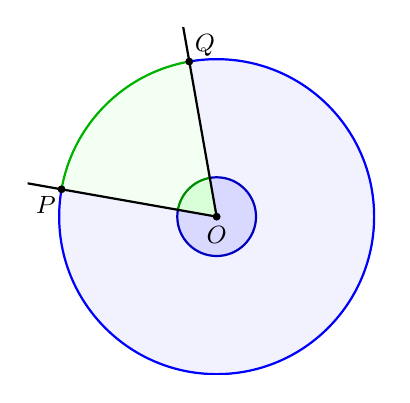
\begin{tikzpicture}[scale=1,font=\small]
\usetikzlibrary{calc}

\begin{scope}
\clip (-2.4,-2.01) rectangle (2.1,2.4);
\coordinate (o) at (0,0);

\draw (o) circle (2);

\path (o) -- (100:2) coordinate (b);
\path (o) -- (170:2) coordinate (a);

\begin{scope}
\clip (a) -- (o) -- (b) -- cycle;
\draw[red, fill=red!10] (o) circle (0.4);
\end{scope}

\begin{scope}
\clip (a) -- (o) -- ++(b) -- ++($(a)-(o)$) -- cycle;
\draw[thick, green!70!black, fill=green!05] (o) circle (2);
\draw[thick, green!55!black, fill=green!15] (o) circle (0.5);
\end{scope}

%\draw[blue] ($(a)!-.25!(o)$) -- (o) -- ++($(b)!-.25!(o)$) -- (2.25,2.25) -- (2.25,-2.25) -- (-2.25,-2.25) -- cycle;

\begin{scope}
\clip ($(a)!-.25!(o)$) -- (o) -- ++($(b)!-.25!(o)$) -- (2.25,2.25) -- (2.25,-2.25) -- (-2.25,-2.25) -- cycle;
\draw[thick, blue, fill=blue!05] (o) circle (2);
\draw[thick, blue!75!black, fill=blue!15] (o) circle (0.5);
\end{scope}

\draw[thick] ($(a)!-.25!(o)$) -- (o) -- ($(b)!-.25!(o)$);

\draw[fill] (a) circle (1.2pt) node[shift={(-0.2,.-0.2)}] {$P$};
\draw[fill] (b) circle (1.2pt) node[shift={(0.2,0.2)}] {$Q$};
\draw[fill] (o) circle (1.2pt) node[below] {$O$};


\end{scope}

\end{tikzpicture}

\end{minipage}

Diamo ora la seguente
\begin{definizione}
Data una circonferenza, si definisce \emph{angolo alla circonferenza} qualsiasi angolo avente il vertice sulla circonferenza e i cui lati siano secanti o tangenti alla circonferenza stessa. 
\end{definizione}
In base alla definizione si possono distinguere tre casi:
\begin{itemize*}
\item i lati dell'angolo sono entrambi secanti alla circonferenza;
\item un lato è secante e l'altro tangente;
\item ambedue i lati sono tangenti.
\end{itemize*}

Anche gli angoli alla circonferenza insistono su archi di circonferenza. Questi appartengono all'angolo stesso e sono delimitati dai punti di tangenza o di intersezione fra i lati dell'angolo e la circonferenza. Nella figura~\ref{fig:ang_circonf} gli angoli alla circonferenza sono segnati in rosso ed i rispettivi archi sono più marcati. Sono invece stati evidenziati in blu i corrispondenti angoli al centro, come segue dalla seguente definizione.

\begin{definizione}
	Un angolo al centro ed un angolo alla circonferenza si dicono \emph{corrispondenti} se insistono sullo stesso arco.
\end{definizione}

\begin{figure}[htb]\label{fig:ang_circonf}
	\centering% Copyright (c) 2015 Daniele Masini - d.masini.it@gmail.com

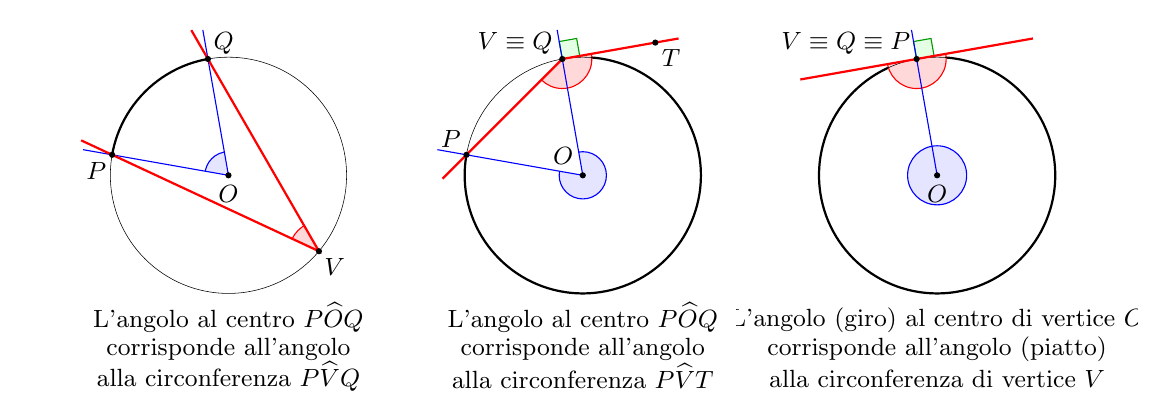
\begin{tikzpicture}[scale=0.75,font=\small]
\usetikzlibrary{calc}

\begin{scope}
\clip (-3.4,-3.65) rectangle (3.4,2.5);
\coordinate (o) at (0,0);

\draw[very thin] (o) circle (2);

\path (o) -- (100:2) coordinate (b);
\path (o) -- (170:2) coordinate (a);
\path (o) -- (320:2) coordinate (c);

\begin{scope}
\clip (a) -- (o) -- (b) -- cycle;
\draw[blue, fill=blue!10] (o) circle (0.4);
\end{scope}

\begin{scope}
\clip ($(a)!-.25!(c)$) -- (c) -- ($(b)!-.25!(c)$) -- cycle;
\draw[thick] (o) circle (2);
\draw[red, fill=red!15] (c) circle (0.5);
\end{scope}

\draw[blue] ($(a)!-.25!(o)$) -- (o) -- ($(b)!-.25!(o)$);
\draw[thick, red] ($(a)!-.15!(c)$) -- (c) -- ($(b)!-.15!(c)$);

\draw[fill] (a) circle (1.2pt) node[shift={(-0.2,.-0.2)}] {$P$};
\draw[fill] (b) circle (1.2pt) node[shift={(0.2,0.2)}] {$Q$};
\draw[fill] (c) circle (1.2pt) node[shift={(0.2,-0.2)}] {$V$};
\draw[fill] (o) circle (1.2pt) node[below] {$O$};

\node at (0,-2.4) {L'angolo al centro $P\widehat{O}Q$};
\node at (0,-2.95) {corrisponde all'angolo};
\node at (0,-3.4) {alla circonferenza $P\widehat{V}Q$};

\end{scope}


\begin{scope}[xshift=6cm]
\clip (-3.4,-3.65) rectangle (3.4,2.5);
%\clip (-2.4,-2.1) rectangle (2.1,2.5);
\coordinate (o) at (0,0);

\path (o) -- (100:2) coordinate (b);
\path (o) -- (170:2) coordinate (a);
\path (b) -- +(10:2) coordinate (d);

\begin{scope}
\clip (a) -- (o) -- (b) -- (2.25,2.25) -- (2.25,-2.25) -- (-2.25,-2.25) -- cycle;
\draw[blue, fill=blue!10] (o) circle (0.4);
\end{scope}

\begin{scope}
\clip ($(a)!-.25!(b)$) -- (b) -- (d) -- (2.25,2.25) -- (2.25,-2.25) -- (-2.25,-2.25) -- cycle;
\draw[thick] (o) circle (2);
\draw[red, fill=red!15] (b) circle (0.5);
\end{scope}

\begin{scope}[rotate=10]
\draw[green!60!black, fill=green!10] (b) rectangle ([shift={(0.3,0.3)}]b);
\end{scope}

\draw[very thin] (o) circle (2);

\draw[blue] ($(a)!-.25!(o)$) -- (o) -- ($(b)!-.25!(o)$);
\draw[thick, red] ($(a)!-.25!(b)$) -- (b) -- (d);

\draw[fill] (a) circle (1.2pt) node[shift={(-0.2,0.2)}] {$P$};
\draw[fill] (b) circle (1.2pt) node[shift={(-0.6,0.2)}] {$V\equiv Q$};
\draw[fill] (o) circle (1.2pt) node[shift={(-0.25,0.25)}] {$O$};
\draw[fill] ($(b)!0.8!(d)$) circle (1.2pt) node[shift={(0.2,-0.2)}] {$T$};

\node at (0,-2.4) {L'angolo al centro $P\widehat{O}Q$};
\node at (0,-2.95) {corrisponde all'angolo};
\node at (0,-3.4) {alla circonferenza $P\widehat{V}T$};
\end{scope}


\begin{scope}[xshift=12cm]
\clip (-3.4,-3.65) rectangle (3.4,2.5);
%\clip (-3.1,-2.1) rectangle (2.1,2.5);
\coordinate (o) at (0,0);

\path (o) -- (100:2) coordinate (b);
\path (b) -- +(10:2) coordinate (d);
\path (b) -- +(190:2) coordinate (e);

\draw[blue, fill=blue!10] (o) circle (0.5);

\begin{scope}
\clip (e) -- (b) -- (d) -- (2.25,2.25) -- (2.25,-2.25) -- (-2.25,-2.25) -- cycle;
\draw[thick] (o) circle (2);
\draw[red, fill=red!15] (b) circle (0.5);
\end{scope}

\begin{scope}[rotate=10]
\draw[green!60!black, fill=green!10] (b) rectangle ([shift={(0.3,0.3)}]b);
\end{scope}

\draw[very thin] (o) circle (2);

\draw[blue] (o) -- ($(b)!-.25!(o)$);
\draw[thick, red] (e) -- (b) -- (d);

\draw[fill] (b) circle (1.2pt) node[shift={(-0.9,0.2)}] {$V\equiv Q\equiv P$};
\draw[fill] (o) circle (1.2pt) node[below] {$O$};

\node at (0,-2.45) {L'angolo (giro) al centro di vertice $O$};
\node at (0,-2.95) {corrisponde all'angolo (piatto)};
\node at (0,-3.45) {alla circonferenza di vertice $V$};

\end{scope}


\end{tikzpicture}

	\caption{Angoli alla circonferenza e corrispondenti angoli al centro}
\end{figure}

\pagebreak

\begin{teorema}
L'angolo alla circonferenza è la metà del corrispondente angolo al centro.
\end{teorema}

\noindent Ipotesi:\tab $\alpha$ angolo alla circonferenza che insiste sull'arco $PQ$;\\
\tab\tab $\beta$ angolo al centro corrispondente ad $\alpha$.\vspace{4pt}\\
Tesi:\tab $\beta = 2\alpha$.

% figura

\begin{proof}
Distinguiamo tre casi:
\begin{enumerate*}
\item Un lato dell'angolo alla circonferenza passa per il centro e dunque si sovrappone al diametro.\\
Abbiamo due possibilità:
\begin{enumerate*}
\noindent\begin{minipage}{0.6\textwidth}\parindent15pt
\item L'altro lato è secante alla circonferenza.\\
Con riferimento alla figura a fianco, il triangolo $OVQ$ è isoscele sulla base $VQ$, in quanto i lati $OV$ e $OQ$ sono due raggi della circonferenza; ne segue che gli angoli alla base sono congruenti e dunque $O\widehat{Q}V\cong \alpha$. L'angolo al centro $P\widehat{O}Q\equiv \beta$ giace sul prolungamento del lato $OV$ e dunque è un angolo esterno al triangolo $OVQ$. Per il teorema degli angoli esterni ad un triangolo, possiamo affermare che $\beta$ è uguale alla somma degli angoli interni non adiacenti e quindi $\beta = \alpha + \alpha = 2\alpha$.
\end{minipage}\hfil
\noindent\hspace{-20pt}\begin{minipage}{0.4\textwidth}
	\centering% Copyright (c) 2015 Daniele Masini - d.masini.it@gmail.com

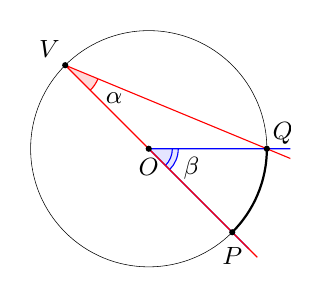
\begin{tikzpicture}[scale=0.75,font=\small]
\usetikzlibrary{calc}

\begin{scope}
\clip (-2.05,-2.05) rectangle (2.4,2.05);
\coordinate (o) at (0,0);

\draw[very thin] (o) circle (2);

\path (o) -- (0:2) coordinate (q);
\path (o) -- (315:2) coordinate (p);
\path (o) -- (135:2) coordinate (v);

\begin{scope}
\clip (p) -- (o) -- (q) -- cycle;
\draw[blue, fill=blue!10] (o) circle (0.5);
\draw[blue] (o) circle (0.4);
\node at ([shift={(335:0.8)}]o) {$\beta$};
\end{scope}

\begin{scope}
\clip ($(p)!-.15!(v)$) -- (v) -- ($(q)!-.15!(v)$) -- cycle;
\draw[thick] (o) circle (2);
\draw[red, fill=red!15] (v) circle (0.6);
\node at ([shift={(326:1)}]v) {$\alpha$};
\end{scope}

\draw[blue] ($(p)!-.2!(o)$) -- (o) -- ($(q)!-.2!(o)$);
\draw[red] ($(p)!-.15!(v)$) -- (v) -- ($(q)!-.15!(v)$);

\draw[fill] (p) circle (1.2pt) node[shift={(0,-0.3)}] {$P$};
\draw[fill] (q) circle (1.2pt) node[shift={(0.2,0.2)}] {$Q$};
\draw[fill] (v) circle (1.2pt) node[shift={(-0.2,0.2)}] {$V$};
\draw[fill] (o) circle (1.2pt) node[below] {$O$};
\end{scope}

\end{tikzpicture}

\end{minipage}
\noindent\begin{minipage}{0.6\textwidth}\parindent15pt
\item L'altro lato è tangente alla circonferenza.\\
In questo caso un lato coincide sempre con il diametro e l'altro è tangente alla circonferenza nel punto $V\equiv Q$; poiché le rette tangenti alla circonferenza sono sempre ortogonali al raggio nel punto di tangenza, i due lati sono perpendicolari. Di conseguenza l'angolo $\alpha$ è un angolo retto e il corrispondente angolo al centro $\beta$ è un angolo piatto, per cui $\beta = 2\alpha$.
\end{minipage}\hfil
\noindent\hspace{-20pt}\begin{minipage}{0.4\textwidth}
	\centering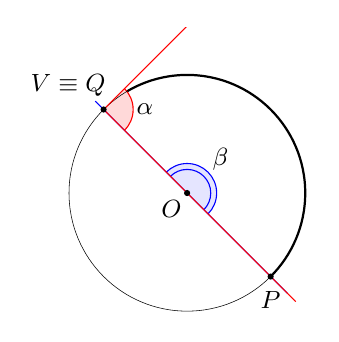
\begin{tikzpicture}[scale=0.75,font=\small]
\usetikzlibrary{calc}

\begin{scope}
\clip (-2.7,-2.05) rectangle (2.1,2.8);
\coordinate (o) at (0,0);

\path (o) -- (135:2) coordinate (q);
\path (o) -- (315:2) coordinate (p);
\path (o) -- (135:2) coordinate (v);
\path (v) -- +(45:2.1) coordinate (t);

\begin{scope}
\clip (p) -- (o) -- (q) -- (0,2.9) -- (2.1,2.1) -- (2.1,-2.1) -- cycle;
\draw[blue, fill=blue!10] (o) circle (0.5);
\draw[blue] (o) circle (0.4);
\node at ([shift={(45:0.8)}]o) {$\beta$};
\end{scope}

\begin{scope}
\clip (p) -- (v) -- (t) -- (2.1,2.1) -- (2.1,-2.1) -- cycle;
\draw[thick] (o) circle (2);
\draw[red, fill=red!15] (v) circle (0.5);
\node at ([shift={(0:0.7)}]v) {$\alpha$};
\end{scope}

\draw[very thin] (o) circle (2);

\draw[blue] ($(p)!-.2!(o)$) -- (o) -- ($(q)!-.1!(o)$);
\draw[red] ($(p)!-.15!(v)$) -- (v) -- (t);

\draw[fill] (p) circle (1.2pt) node[shift={(0,-0.3)}] {$P$};
\draw[fill] (v) circle (1.2pt) node[shift={(-0.45,0.3)}] {$V\equiv Q$};
\draw[fill] (o) circle (1.2pt) node[shift={(-0.2,-0.2)}] {$O$};
\end{scope}

\end{tikzpicture}

\end{minipage}
\end{enumerate*}

\item Il centro $O$ è interno all'angolo alla circonferenza.\\
Anche in questo caso abbiamo due possibilità:
\begin{enumerate*}
\noindent\begin{minipage}{0.6\textwidth}\parindent15pt
\item I lati dell'angolo alla circonferenza sono entrambi secanti.\\
Si conduca dal vertice $V$ dell'angolo alla circonferenza $P\widehat{V}Q$ il diametro $VT$; si ottengono in tal modo due angoli alla circonferenza $P\widehat{V}T$ e $T\widehat{V}Q$ la cui somma è proprio l'angolo $P\widehat{V}Q$. Tali angoli hanno il lato comune il lato $VT$ coincidente con il diametro e dunque, essendo $P\widehat{O}T$ e $T\widehat{O}Q$ i rispettivi angoli al centro, possiamo applicare ad ognuno di essi il risultato dimostrato al punto 1: $P\widehat{O}T=2P\widehat{V}T$ e $T\widehat{O}Q=2T\widehat{V}Q$.
Ma la somma degli angoli $P\widehat{O}T$ e $T\widehat{O}Q$ è pari all'angolo al centro $P\widehat{O}Q$, corrispondente all'angolo alla circonferenza $P\widehat{V}Q$.
Dunque $P\widehat{O}Q=P\widehat{O}T+T\widehat{O}Q=2P\widehat{V}T+2T\widehat{V}Q=2(P\widehat{V}T+T\widehat{V}Q)=2P\widehat{V}Q$.
\end{minipage}\hfil
\noindent\hspace{-20pt}\begin{minipage}{0.4\textwidth}
	\centering% Copyright (c) 2015 Daniele Masini - d.masini.it@gmail.com

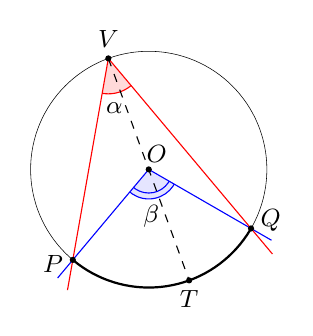
\begin{tikzpicture}[scale=0.75,font=\small]
\usetikzlibrary{calc}

\begin{scope}
\clip (-2.05,-2.35) rectangle (2.3,2.4);
\coordinate (o) at (0,0);

\path (o) -- (330:2) coordinate (q);
\path (o) -- (230:2) coordinate (p);
\path (o) -- (110:2) coordinate (v);

\begin{scope}
\clip (p) -- (o) -- (q) -- cycle;
\draw[blue, fill=blue!10] (o) circle (0.5);
\draw[blue] (o) circle (0.4);
\node at ([shift={(273:0.8)}]o) {$\beta$};
\end{scope}

\begin{scope}
\clip ($(p)!-.15!(v)$) -- (v) -- ($(q)!-.15!(v)$) -- (280:2.3) -- cycle;
\draw[thick] (o) circle (2);
\draw[red, fill=red!15] (v) circle (0.6);
\node at ([shift={(277:0.85)}]v) {$\alpha$};
\end{scope}

\draw[dashed] (v) -- ($(v)!2!(o)$) coordinate (t);
\draw[fill] (t) circle (1.2pt) node[below] {$T$};

\draw[very thin] (o) circle (2);

\draw[blue] ($(p)!-.2!(o)$) -- (o) -- ($(q)!-.2!(o)$);
\draw[red] ($(p)!-.15!(v)$) -- (v) -- ($(q)!-.15!(v)$);

\draw[fill] (p) circle (1.2pt) node[shift={(-0.25,-0.05)}] {$P$};
\draw[fill] (q) circle (1.2pt) node[shift={(0.25,0.1)}] {$Q$};
\draw[fill] (v) circle (1.2pt) node[shift={(0,0.25)}] {$V$};
\draw[fill] (o) circle (1.2pt) node[shift={(0.1,0.2)}] {$O$};
\end{scope}

\end{tikzpicture}

\end{minipage}
\noindent\begin{minipage}{0.6\textwidth}\parindent15pt
\item Un lato dell'angolo alla circonferenza è tangente.\\
La dimostrazione è del tutto simile alla precedente. Il diametro $VC$ divide l'angolo alla circonferenza $P\widehat{V}T$ negli angoli $P\widehat{V}C$ e $C\widehat{V}T$. Per il primo angolo vale quanto già dimostrato al punto 1a e ribadito al punto precedente: detto $P\widehat{O}C$ il corrispondente angolo al centro, possiamo scrivere $P\widehat{O}C=2P\widehat{V}C$. Inoltre, $C\widehat{V}T$ è retto per costruzione e difatti misura la metà del corrispondente angolo al centro $C\widehat{O}V$, che è proprio un angolo piatto (vedi quanto dimostrato nel punto 1b). Anche in questo caso, essendo $P\widehat{O}V$ l'angolo al centro corrispondente all'angolo $P\widehat{V}T$, si dimostra che $P\widehat{O}V=P\widehat{O}C+T\widehat{O}Q=2P\widehat{V}C+2C\widehat{V}T=2(P\widehat{V}C+C\widehat{V}T)=2P\widehat{V}T$.
Si noti che $P\widehat{O}V$ è un angolo concavo, ovvero maggiore di un angolo piatto.
\end{minipage}\hfil
\noindent\hspace{-20pt}\begin{minipage}{0.4\textwidth}
	\centering% (c) 2014 Daniele Masini - d.masini.it@gmail.com
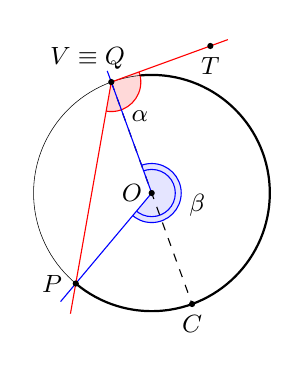
\begin{tikzpicture}[scale=0.75,font=\small]
\usetikzlibrary{calc}

\begin{scope}
\clip (-2.1,-2.45) rectangle (2.1,2.8);
\coordinate (o) at (0,0);

\path (o) -- (110:2) coordinate (q);
\path (o) -- (230:2) coordinate (p);
\path (o) -- (110:2) coordinate (v);
\path (v) -- +(20:2.1) coordinate (t);

\begin{scope}
\clip (p) -- (o) -- (q) -- (0,2.9) -- (2.1,2.1) -- (2.1,-2.1) -- cycle;
\draw[blue, fill=blue!10] (o) circle (0.5);
\draw[blue] (o) circle (0.4);
\node at ([shift={(-15:0.8)}]o) {$\beta$};
\end{scope}

\begin{scope}
\clip (p) -- (v) -- (t) -- (2.1,2.1) -- (2.1,-2.1) -- (-2.1,-2.1) -- cycle;
\draw[thick] (o) circle (2);
\draw[red, fill=red!15] (v) circle (0.5);
\node at ([shift={(-50:0.75)}]v) {$\alpha$};
\end{scope}

\draw[dashed] (v) -- ($(v)!2!(o)$) coordinate (c);
\draw[very thin] (o) circle (2);

\draw[blue] ($(p)!-.2!(o)$) -- (o) -- ($(q)!-.1!(o)$);
\draw[red] ($(p)!-.15!(v)$) -- (v) -- (t);

\draw[fill] (c) circle (1.2pt) node[shift={(0,-0.25)}] {$C$};
\draw[fill] ($(v)!0.85!(t)$) circle (1.2pt) node[shift={(0,-0.25)}] {$T$};
\draw[fill] (p) circle (1.2pt) node[shift={(-0.3,0)}] {$P$};
\draw[fill] (v) circle (1.2pt) node[shift={(-0.3,0.3)}] {$V\equiv Q$};
\draw[fill] (o) circle (1.2pt) node[shift={(-0.25,0)}] {$O$};
\end{scope}

\end{tikzpicture}

\end{minipage}
\end{enumerate*}

\item Il centro $O$ è esterno all'angolo alla circonferenza.\\
Anche qui abbiamo due casi:
\begin{enumerate*}
\noindent\begin{minipage}{0.6\textwidth}\parindent15pt
\item Entrambi i lati dell'angolo alla circonferenza sono secanti.\\
Sia $P\widehat{V}Q$ l'angolo alla circonferenza. Tracciamo il diametro $VT$. Per quanto dimostrato al punto 1.a, l'angolo al centro $T\widehat{O}Q$ è il doppio del corrispondente angolo alla circonferenza $T\widehat{V}Q$ e $T\widehat{O}P$ è il doppio dell'angolo $T\widehat{V}P$. Essendo $P\widehat{O}Q$ l'angolo al centro corrispondente a quello alla circonferenza $P\widehat{V}Q$, possiamo  scrivere: $P\widehat{O}Q=T\widehat{O}Q-T\widehat{O}P=2T\widehat{V}Q-2T\widehat{V}P=2(T\widehat{V}Q+T\widehat{V}P)=2P\widehat{V}Q$.
\end{minipage}\hfil
\noindent\hspace{-20pt}\begin{minipage}{0.4\textwidth}
	\centering% (c) 2014 Daniele Masini - d.masini.it@gmail.com
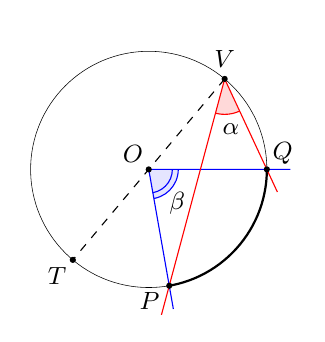
\begin{tikzpicture}[scale=0.75,font=\small]
\usetikzlibrary{calc}

\begin{scope}
\clip (-2.05,-2.45) rectangle (2.5,2.4);
\coordinate (o) at (0,0);

\path (o) -- (0:2) coordinate (q);
\path (o) -- (-80:2) coordinate (p);
\path (o) -- (50:2) coordinate (v);

\begin{scope}
\clip (p) -- (o) -- (q) -- cycle;
\draw[blue, fill=blue!10] (o) circle (0.5);
\draw[blue] (o) circle (0.4);
\node at ([shift={(-50:0.75)}]o) {$\beta$};
\end{scope}

\begin{scope}
\clip ($(p)!-.15!(v)$) -- (v) -- ($(q)!-.15!(v)$) -- (320:2.3) -- cycle;
\draw[thick] (o) circle (2);
\draw[red, fill=red!15] (v) circle (0.6);
\node at ([shift={(277:0.85)}]v) {$\alpha$};
\end{scope}

\draw[dashed] (v) -- ($(v)!2!(o)$) coordinate (t);
\draw[fill] (t) circle (1.2pt) node[shift={(-0.2,-0.2)}] {$T$};

\draw[very thin] (o) circle (2);

\draw[blue] ($(p)!-.2!(o)$) -- (o) -- ($(q)!-.2!(o)$);
\draw[red] ($(p)!-.15!(v)$) -- (v) -- ($(q)!-.25!(v)$);

\draw[fill] (p) circle (1.2pt) node[shift={(-0.25,-0.2)}] {$P$};
\draw[fill] (q) circle (1.2pt) node[shift={(0.2,0.2)}] {$Q$};
\draw[fill] (v) circle (1.2pt) node[shift={(0,0.25)}] {$V$};
\draw[fill] (o) circle (1.2pt) node[shift={(-0.2,0.2)}] {$O$};
\end{scope}

\end{tikzpicture}

\end{minipage}
\noindent\begin{minipage}{0.6\textwidth}\parindent15pt
\item Un lato dell'angolo alla circonferenza è tangente.\\
La dimostrazione è analoga alla precedente e fa uso delle proprietà 1.a e 1.b. Tracciato il diametro $VC$, essendo $P\widehat{O}V$ l'angolo al centro corrispondente a quello alla circonferenza $P\widehat{V}T$, possiamo scrivere: $P\widehat{O}V=C\widehat{O}V-C\widehat{O}P=2C\widehat{V}T-2C\widehat{V}P=2(C\widehat{V}T+C\widehat{V}P)=2P\widehat{V}T$.
\end{minipage}\hfil
\noindent\hspace{-20pt}\begin{minipage}{0.4\textwidth}
	\centering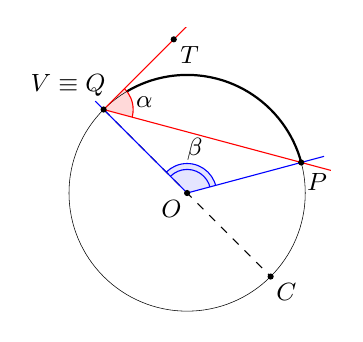
\begin{tikzpicture}[scale=0.75,font=\small]
\usetikzlibrary{calc}

\begin{scope}
\clip (-2.7,-2.05) rectangle (2.5,2.8);
\coordinate (o) at (0,0);

\path (o) -- (135:2) coordinate (q);
\path (o) -- (15:2) coordinate (p);
\path (o) -- (135:2) coordinate (v);
\path (v) -- +(45:2.1) coordinate (t);

\begin{scope}
\clip (p) -- (o) -- (q) -- (0,2.9) -- (2.1,2.1) -- (2.1,-2.1) -- cycle;
\draw[blue, fill=blue!10] (o) circle (0.5);
\draw[blue] (o) circle (0.4);
\node at ([shift={(80:0.75)}]o) {$\beta$};
\end{scope}

\begin{scope}
\clip (p) -- (v) -- (t) -- (2.1,2.1) -- cycle;
\draw[thick] (o) circle (2);
\draw[red, fill=red!15] (v) circle (0.5);
\node at ([shift={(10:0.7)}]v) {$\alpha$};
\end{scope}

\draw[dashed] (v) -- ($(v)!2!(o)$) coordinate (c);
\draw[very thin] (o) circle (2);

\draw[blue] ($(p)!-.2!(o)$) -- (o) -- ($(q)!-.1!(o)$);
\draw[red] ($(p)!-.15!(v)$) -- (v) -- (t);

\draw[fill] (c) circle (1.2pt) node[shift={(0.2,-0.2)}] {$C$};
\draw[fill] ($(v)!0.8!(t)$) circle (1.2pt) node[shift={(0.2,-0.2)}] {$T$};
\draw[fill] (p) circle (1.2pt) node[shift={(0.2,-0.25)}] {$P$};
\draw[fill] (v) circle (1.2pt) node[shift={(-0.45,0.3)}] {$V\equiv Q$};
\draw[fill] (o) circle (1.2pt) node[shift={(-0.2,-0.2)}] {$O$};
\end{scope}

\end{tikzpicture}

\end{minipage}
\end{enumerate*}
\end{enumerate*}
\end{proof}

I seguenti corollari sono immediata conseguenza del precedente teorema.
\begin{corollario}
Angoli alla circonferenza che insistono su uno stesso arco sono congruenti.
\end{corollario}

\noindent\begin{minipage}{0.6\textwidth}\parindent15pt
\begin{proof}
Gli angoli alla circonferenza che nelle figura a lato insistono sullo stesso arco $PQ$ misurano tutti la metà del corrispondente angolo al centro $P\widehat{O}Q$. Quindi sono tra loro congruenti.
\end{proof}
\end{minipage}\hfil
\noindent\begin{minipage}{0.4\textwidth}
	\centering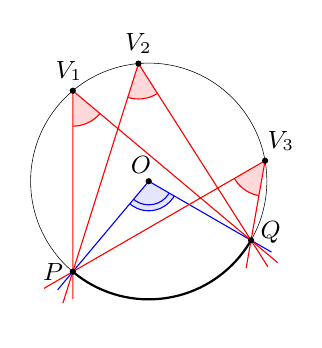
\begin{tikzpicture}[scale=0.75,font=\small]
\usetikzlibrary{calc}

\begin{scope}
\clip (-2.05,-2.35) rectangle (2.45,2.6);
\coordinate (o) at (0,0);

\path (o) -- (330:2) coordinate (q);
\path (o) -- (230:2) coordinate (p);
\path (o) -- (130:2) coordinate (v);
\path (o) -- (95:2) coordinate (s);
\path (o) -- (10:2) coordinate (t);

\begin{scope}
\clip (p) -- (o) -- (q) -- cycle;
\draw[blue, fill=blue!10] (o) circle (0.5);
\draw[blue] (o) circle (0.4);
\end{scope}

\begin{scope}
\clip ($(p)!-.15!(v)$) -- (v) -- ($(q)!-.15!(v)$) -- (280:2.3) -- cycle;
\draw[thick] (o) circle (2);
\draw[red, fill=red!15] (v) circle (0.6);
\end{scope}

\begin{scope}
\clip ($(p)!-.15!(s)$) -- (s) -- ($(q)!-.15!(s)$) -- (280:2.3) -- cycle;
\draw[red, fill=red!15] (s) circle (0.6);
\end{scope}

\begin{scope}
\clip ($(p)!-.15!(t)$) -- (t) -- ($(q)!-.15!(t)$) -- (280:2.3) -- cycle;
\draw[red, fill=red!15] (t) circle (0.6);
\end{scope}

\draw[very thin] (o) circle (2);

\draw[blue] ($(p)!-.2!(o)$) -- (o) -- ($(q)!-.2!(o)$);
\draw[red] ($(p)!-.15!(v)$) -- (v) -- ($(q)!-.15!(v)$);
\draw[red] ($(p)!-.15!(s)$) -- (s) -- ($(q)!-.15!(s)$);
\draw[red] ($(p)!-.15!(t)$) -- (t) -- ($(q)!-.35!(t)$);

\draw[fill] (p) circle (1.2pt) node[shift={(-0.25,0)}] {$P$};
\draw[fill] (q) circle (1.2pt) node[shift={(0.25,0.1)}] {$Q$};
\draw[fill] (v) circle (1.2pt) node[shift={(-0.05,0.25)}] {$V_1$};
\draw[fill] (s) circle (1.2pt) node[shift={(0,0.25)}] {$V_2$};
\draw[fill] (t) circle (1.2pt) node[shift={(0.2,0.25)}] {$V_3$};
\draw[fill] (o) circle (1.2pt) node[shift={(-0.1,0.2)}] {$O$};
\end{scope}

\end{tikzpicture}

\end{minipage}

\begin{corollario}
Ogni angolo alla circonferenza che insiste su una semicirconferenza è retto.
\end{corollario}
\noindent\begin{minipage}{0.6\textwidth}\parindent15pt
\begin{proof}
Il corrispondente angolo al centro è infatti un angolo piatto.
\end{proof}
\end{minipage}\hfil
\noindent\begin{minipage}{0.4\textwidth}
	\centering% (c) 2014 Daniele Masini - d.masini.it@gmail.com
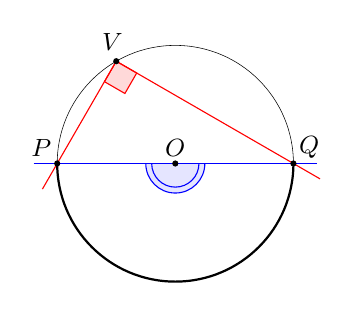
\begin{tikzpicture}[scale=0.75,font=\small]
\usetikzlibrary{calc}

\begin{scope}
\clip (-2.5,-2.05) rectangle (2.5,2.3);
\coordinate (o) at (0,0);

\path (o) -- (0:2) coordinate (q);
\path (o) -- (180:2) coordinate (p);
\path (o) -- (120:2) coordinate (v);

\begin{scope}
\clip (p) -- (o) -- (q) -- (270:2) -- cycle;
\draw[blue, fill=blue!10] (o) circle (0.5);
\draw[blue] (o) circle (0.4);
\end{scope}

\begin{scope}
\clip ($(p)!-.15!(v)$) -- (v) -- ($(q)!-.15!(v)$) -- (300:2.5) -- (235:2.5) -- cycle;
\draw[thick] (o) circle (2);
%\draw[red, fill=red!15] (v) circle (0.6);
\end{scope}

\begin{scope}[rotate=240]
\draw[red, fill=red!15] (v) rectangle ([shift={(0.4,0.4)}]v);
\end{scope}


\draw[very thin] (o) circle (2);

\draw[blue] ($(p)!-.2!(o)$) -- (o) -- ($(q)!-.2!(o)$);
\draw[red] ($(p)!-.25!(v)$) -- (v) -- ($(q)!-.15!(v)$);

\draw[fill] (p) circle (1.2pt) node[shift={(-0.2,0.2)}] {$P$};
\draw[fill] (q) circle (1.2pt) node[shift={(0.2,0.2)}] {$Q$};
\draw[fill] (v) circle (1.2pt) node[shift={(-0.05,0.25)}] {$V$};
\draw[fill] (o) circle (1.2pt) node[shift={(0,0.2)}] {$O$};
\end{scope}

\end{tikzpicture}

\end{minipage}

Premesso che affinché due circonferenze siano congruenti è sufficiente che abbiano lo stesso raggio, sussistono i seguenti teoremi, di cui lasciamo la dimostrazione al lettore che può essere effettuata velocemente ricorrendo alla sovrapposizione tramite movimento rigido degli elementi dei quali si vuole dimostrare la congruenza (in una stessa circonferenza questo si otterrà tramite rotazione intorno al centro).

\begin{teorema}
In una stessa circonferenza o in circonferenze congruenti
\begin{itemize*}
\item ad archi congruenti corrispondono angoli al centro e corde congruenti;
\item a corde congruenti corrispondono angoli al centro ed archi congruenti;
\item ad angoli al centro congruenti corrispondono archi e corde congruenti.
\end{itemize*}
\end{teorema}

\section{Proprietà dei segmenti di tangenza}

Data una circonferenza $C$ di centro $O$ e raggio $r$, ed un punto $P$ del piano, quante sono le rette passanti per $P$ e tangenti a $C$?  Ovviamente, dipende dalla posizione del punto $P$ rispetto alla circonferenza $C$. Se $P$ è interno a $C$, non esiste alcuna retta passante per $P$ e tangente a $C$, anche perché $OP < r$. Se invece il punto $P\in C$, allora esiste una ed una sola retta passante per $P$ e tangente a $C$ ed in questo caso $OP$ coincide con un raggio di $C$ e la retta tangente è perpendicolare ad $OP$.
Se consideriamo un punto $P$ esterno a $C$, allora esistono due rette distinte passanti per $P$ e tangenti a $C$. Verifichiamo, con l'aiuto di una costruzione geometrica, che da un punto esterno ad una circonferenza possiamo tracciare due tangenti, e due sole, alla circonferenza stessa.
Uniamo $P$ con $O$ e costruiamo la circonferenza di diametro $OP$; le due circonferenze si intersecano in due punti distinti $A$ e $B$. Uniamo $A$ e $B$ con $O$ e con $P$. Gli angoli $O\widehat{A}P$ e $O\widehat{B}P$ sono retti perché sono angoli alla circonferenza che insistono su semicirconferenze. Dunque $OA\perp AP$ e $OB\perp BP$, per cui le rette $AP$ e $BP$ hanno distanza da $O$ pari ad $r$, e quindi sono tangenti a $C$. $A$ e $B$ sono gli unici punti per cui valgono le relazioni precedenti, perché sono gli unici punti di intersezione delle due circonferenze. $AP$ e $BP$ sono pertanto le due uniche rette passanti per $P$ e tangenti a $C$.

I segmenti $AP$ e $BP$ che uniscono i punti di tangenza con il punto esterno $P$ sono detti \emph{segmenti tangenti}.

\begin{teorema}
I segmenti tangenti condotti da un punto $P$ ad una circonferenza sono congruenti.
\end{teorema}

\begin{proof}
Infatti, seguendo le linee della costruzione precedente, i triangoli rettangoli $OPA$ e $OPB$ hanno l'ipotenusa $OP$ in comune e i cateti $OA$ e $OB$ congruenti perché raggi della stessa circonferenza; sono dunque congruenti per il criterio particolare dei triangoli rettangoli e di conseguenza gli altri due cateti $AP$ e $BP$ risultano congruenti, come volevasi dimostrare.
\end{proof}

Dalla congruenza dei due triangoli rettangoli segue anche la congruenza delle due coppie di angoli acuti: $A\widehat{O}P\cong B\widehat{O}P$ e $A\widehat{P}O\cong B\widehat{P}O$. Da queste due congruenze segue il seguente 
\begin{corollario}
Il segmento che unisce il centro di una circonferenza con un punto esterno $P$ è bisettrice sia dell'angolo formato dalle due tangenti uscenti da $P$ sia dell'angolo al centro avente come lati i raggi per i punti di tangenza.
\end{corollario}
Inoltre, esso è anche perpendicolare alla corda avente per estremi i punti di tangenza.

\begin{corollario}
Date due circonferenze secanti, la congiungente dei loro centri è perpendicolare alla congiungente dei punti di intersezione.
\end{corollario}

Lasciamo al lettore la dimostrazione.

Abbiamo definito \emph{asse radicale} la retta passante per i due punti di intersezione di due circonferenze, ma si parla di asse radicale in maniera più generale, cioè anche nel caso di due circonferenze tra loro non sono secanti. L'asse radicale non esiste soltanto nel caso in cui le due circonferenze siano concentriche.
Nel caso in cui le due circonferenze siano tangenti (sia esternamente o internamente), l'asse radicale coincide con la tangente in comune.
Nel caso in cui le due circonferenze non abbiano punti in comune (reciprocamente esterne, o l'una interna all'altra, ma non concentriche), l'asse radicale è una particolare retta esterna ad entrambe, perpendicolare alla congiungente dei centri, e luogo geometrico dei punti tali che, tracciando da essi i segmenti tangenti alle due circonferenze essi risultano congruenti.


\section{Poligoni inscritti e circoscritti ad una circonferenza}

\begin{definizione}
Un poligono si dice \emph{inscritto in una circonferenza} se tutti i vertici del poligono appartengono alla circonferenza.
\end{definizione}

\begin{definizione}
Un poligono si dice \emph{circoscritto a una circonferenza} se tutti i suoi lati sono tangenti alla circonferenza.
\end{definizione}

\begin{teorema}
Se un poligono ha gli assi dei lati che si incontrano tutti in uno stesso punto allora il poligono può essere inscritto in una circonferenza, e viceversa se un poligono è inscritto in una circonferenza allora gli assi dei suoi lati si incontrano tutti nel centro della circonferenza.
\end{teorema}

\begin{proof}~\\
\begin{enumerate*}
\item Dimostrazione diretta.\\
Sia $ABCDEF$ un poligono che ha gli assi dei suoi lati che passano per uno stesso punto $O$. Poiché $O$ appartiene all'asse di $AB$ e poiché l'asse è il luogo dei punti equidistanti dagli estremi, si ha che $OA\cong OB$. Poiché $O$ appartiene anche all'asse di $BC$ allora $O$ è equidistante dagli estremi di $BC$, cioè $OB\cong OC$. Poiché ciò vale per tutti i lati del poligono si ha: $OA\cong OB\cong OC\cong OD\cong OE\cong OF$. Pertanto la circonferenza di centro $O$ e raggio $OA$ passa per tutti i vertici del poligono e il poligono risulta pertanto inscritto in essa.
\item Dimostrazione inversa.\\
Sia $ABCDEF$ un poligono inscritto in una circonferenza e che ha quindi tutti i vertici sulla circonferenza, allora tutti i suoi lati sono corde della circonferenza, di conseguenza, per una proprietà delle corde, gli assi delle corde passano per il centro della circonferenza, e quindi tutti gli assi dei lati del poligono si incontrano nel centro della circonferenza.
\end{enumerate*}
\end{proof}

\begin{teorema}
Se un poligono convesso ha le bisettrici degli angoli che passano tutte per uno stesso punto allora il poligono può essere circoscritto a una circonferenza, e viceversa se il poligono è circoscritto a una circonferenza allora tutte le bisettrici degli angoli del poligono passano per il centro della circonferenza.
\end{teorema}

\begin{proof}
Sia $ABCD$ il poligono convesso; $AO$ la bisettrice dell'angolo in $A$ e $BO$ quella dell'angolo in $B$. Poiché la bisettrice è il luogo dei punti equidistanti dai lati dell'angolo, si ha che il punto $O$ è equidistante dal lato $AD$ e dal lato $AB$, cioè $OH\cong OK$. Analogamente, $O$, appartenendo alla bisettrice $BO$ dell'angolo in $B$, è equidistante da $AB$ e da $BC$, cioè $OJ\cong OK$. Ciò vale per tutti i lati del poligono, pertanto $OH\cong OK\cong OJ\cong \ldots$. Tracciando la circonferenza di centro $O$ e raggio $OH$ si ha la circonferenza alla quale il poligono risulta circosritto.
La dimostrazione del teorema inverso si basa anch’essa sulla proprietà della bisettrice dell’angolo.
\end{proof}


\section{Punti notevoli di un triangolo}

\subsection{Circocentro}

I vertici di un triangolo sono tre punti non allineati, dunque per essi passa una ed una sola circonferenza: il centro di tale circonferenza si trova come intersezione degli assi di due lati del triangolo. Il centro della circonferenza circoscritta al triangolo è appunto detto \emph{circocentro} del triangolo.
\begin{teorema}
I tre assi dei lati di un triangolo si incontrano nel suo circocentro.
\end{teorema}

\begin{proof}
Sia $ABC$ un triangolo e siano $e$ l'asse di $AB$, $d$ l'asse di $BC$ ed $f$ l'asse di $AC$. Sia $D$ il punto di intersezione tra $d$ ed $e$ (che, come detto in precedenza, esiste perché le due rette, in quanto perpendicolari a due segmenti non paralleli, non possono essere parallele). Allora risulta $AB\cong BD$ in quanto $D\in e$, ed anche $BC\cong CD$ in quanto $P\in d$; dunque, per la proprietà transitiva della congruenza, risulta $AD\cong CD$ e quindi $P\in f$. Pertanto $D$ risulta equidistante dai tre vertici ed è quindi il centro della circonferenza circoscritta.
\end{proof}

\osservazione Il circocentro di un triangolo può essere interno o esterno al triangolo o sul perimetro. Ricordando le proprietà degli angoli alla circonferenza, il circocentro è sul perimetro solo nel caso in cui il triangolo è rettangolo, ed in tal caso si trova sul punto medio dell'ipotenusa.
Da ciò seguono le seguenti importanti proprietà:
\begin{teorema}
In un triangolo rettangolo
\begin{itemize*}
\item il punto medio dell'ipotenusa è equidistante dai tre vertici;
\item la mediana relativa all'ipotenusa è congruente alla metà dell'ipotenusa stessa.
\end{itemize*}
\end{teorema}

Sempre per le proprietà degli angoli alla circonferenza, il circocentro di un triangolo è interno al triangolo se il triangolo è acutangolo, mentre è esterno se il triangolo è ottusangolo (il corrispondente angolo al centro è rispettivamente convesso o concavo).

\subsection{Incentro}

Esiste uno ed un solo punto equidistante dai tre lati di un triangolo, pertanto un triangolo è sempre circoscrivibile ad una circonferenza, cioè esiste ed è unica la circonferenza inscritta in un triangolo ed il suo centro è detto \emph{incentro} del triangolo.

\begin{teorema}
Le bisettrici dei tre angoli di un triangolo si incontrano nel suo incentro.
\end{teorema}

\begin{proof}
Ricordiamo che la bisettrice è la semiretta che divide a metà l'angolo e quindi è anche il luogo dei punti equidistanti dai lati dell'angolo. Consideriamo un triangolo $ABC$ ed i suoi tre angoli interni. Poiché la somma degli angoli interni di un triangolo è un angolo piatto ($\pi$), abbiamo $\widehat{A}+\widehat{B}<\pi$ e a maggior ragione $\frac{1}{2}\widehat{A}+\frac{1}{2}\widehat{B}<\pi$. Quindi poiché i lati $AC$ e $BC$ non sono paralleli a maggior ragione non possono essere parallele le bisettrici degli angoli interni di vertici $A$ e $B$, anzi i segmenti di bisettrice sono certamente interni al triangolo. Detto $D$ il punto di intersezione delle bisettrici di $\widehat{A}$ e di $\widehat{B}$, verifichiamo che anche la bisettrice di $\widehat{C}$ passa per $D$. Poiché $D$ appartiene alla bisettrice di $\widehat{A}$, è equidistante dai lati $AB$ e $AC$ ($GD\cong DE$); analogamente, poiché $D$ appartiene alla bisettrice di $\widehat{B}$, è equidistante dai lati $AB$ e $BC$ ($GD\cong DF$). Dunque $Q$ deve essere equidistante dai lati $AC$ e $BC$, pertanto $D$ deve appartenere alla bisettrice di $\widehat{C}$. La distanza comune di $D$ dai tre lati è il raggio della circonferenza inscritta nel triangolo, che ha centro $D$.
\end{proof}

\subsection{Ortocentro}

Un altro punto notevole di un triangolo è il punto di incontro delle altezze, detto \emph{ortocentro}. Anche questo esiste ed è unico. Ricordiamo che di solito si parla di altezza come del segmento che unisce un vertice con il piede della perpendicolare al lato opposto. Qui ci occupiamo di retta dell'altezza, cioè della retta perpendicolare ad un lato di un triangolo e passante per il vertice opposto. Osserviamo infatti che, mentre l'incentro è certamente interno al triangolo, l'ortocentro può essere esterno.

\begin{teorema}
Le tre altezze di un triangolo si incontrano nel suo ortocentro.
\end{teorema}

% figura

\begin{proof}
Sia $ABC$ un triangolo. Tracciamo la retta parallela a $BC$ e passante per $A$; analogamente tracciamo la parallela ad $AC$ passante per $B$ e la parallela ad $AB$ passante per $C$. Le tre rette, essendo parallele ai tre lati del triangolo $ABC$, sono a due a due incidenti. Chiamiamo $A'$ il punto di intersezione tra $AB$ ed $AC$, $B'$ il punto di intersezione tra $AB$ e $BC$ e $C'$ il punto di intersezione tra $AC$ e $BC$.

Il triangolo $BCA'$ risulta congruente al triangolo $ABC$ per il secondo criterio, in quanto ha BC in comune, $A\widehat{C}B\cong C\widehat{B}A$ e $A\widehat{B}C\cong B\widehat{C}A$ perché angoli alterni interni tra coppie di rette parallele tagliate dalla trasversale $BC$. Analogamente anche i triangoli $ABC'$ e $ACB'$ risultano congruenti ad $ABC$ per il secondo criterio, quindi i quattro triangoli sono tutti congruenti. In particolare risulta che i segmenti $C'A$, $AB'$ e $BC$ sono paralleli e congruenti, dunque la retta passante per $A$ e perpendicolare a $BC$ è sia l'altezza del triangolo $ABC$ relativa al lato $BC$ sia l'asse del segmento $C'B'$. Lo stesso vale per le altre due altezze. Dunque le tre altezze del triangolo $ABC$ coincidono con gli assi dei lati del triangolo $A'B'C'$: quindi l'ortocentro di $ABC$ esiste perché coincide con il circocentro di $A'B'C'$.
\end{proof}

\begin{osservazione}
Dalla costruzione precedente, risulta, pertanto $ABC$ è acutangolo, rettangolo, ottusangolo come $A'B'C'$. Possiamo affermare dunque che:
\begin{itemize*}
\item se $ABC$ è rettangolo lo è pure $A'B'C'$ ed il punto medio dell'ipotenusa di $A'B'C'$ coincide con il vertice dell'angolo retto di $ABC$;
\item se $ABC$ è ottusangolo il suo circocentro è esterno ad esso, quindi l'ortocentro di $ABC$, dovendo essere esterno al triangolo $A'B'C'$, è a maggior ragione esterno ad $ABC$;
\item se $ABC$ è acutangolo quanto detto in precedenza ci permette solo di affermare che il circocentro di $A'B'C'$, che è anche l'ortocentro di $ABC$, è interno ad $A'B'C'$, ma in realtà è interno anche ad $ABC$.
\end{itemize*}
Questo si vede meglio se consideriamo il classico modo di disegnare l'altezza: facciamo eventualmente compiere al triangolo una rototraslazione in modo che il lato rispetto al quale vogliamo tracciare l'altezza sia ``orizzontale'' ed il vertice opposto si trovi nel ``semipiano in alto''; se il triangolo è acutangolo, comunque scegliamo il lato rispetto al quale vogliamo tracciare l'altezza, gli angoli compresi sono entrambi acuti, per cui il piede dell'altezza deve essere necessariamente interno al lato, e pertanto l'intera altezza (segmento) deve essere interna al triangolo. Come nel caso dell'incentro, che è sempre interno al triangolo, anche l'ortocentro è interno nel caso di triangolo ottusangolo. Lasciamo al lettore la dimostrazione dettagliata di queste due affermazioni (si può procedere per assurdo), ed illustriamo quanto detto nella figura seguente.
In riferimento alla figura del teorema precedente, l'ortocentro del triangolo $ABC$, e quindi anche il circocentro del triangolo $A'B'C'$, non può cadere all'interno di uno dei triangoli $ABC'$, $AB'C$ e $A'BC$. 
\end{osservazione}

\subsection{Baricentro}

Si chiama \emph{baricentro} di un triangolo il punto di incontro delle tre mediane. Poiché le mediane sono segmenti interni ad un triangolo, anche il baricentro lo è (segue banalmente dal teorema seguente che, oltre a dirci che il baricentro esiste ed è unico, ci dà anche un modo ``operativo'' per individuarlo).

\begin{teorema}[del baricentro]
Le tre mediane di un triangolo si incontrano in un punto, detto baricentro, che divide ciascuna di esse in due parti tali che una (quella che contiene il vertice) è doppia dell'altra.
\end{teorema}

\begin{proof}
Si tratta di una delle principali conseguenze della corrispondenza di Talete, segue in particolare dal corollario riguardante i segmenti che uniscono i punti medi dei lati di un triangolo e dalle proprietà dei parallelogrammi.

Dimostriamo prima che la tesi è verificata per il punto di intersezione di due mediane, e poi dimostriamo che la terza mediana passa per quel punto.
Sia $ABC$ un triangolo. Detti $D$, $E$ ed $F$ i punti medi rispettivamente dei lati $AC$, $BC$ ed $AB$, tracciamo le mediane $AE$ e $BD$. Queste, essendo interne al triangolo, certamente si incontreranno in un punto che chiamiamo $G$. Chiamiamo inoltre $H$ il punto medio del segmento $AG$ ed $M$ il punto medio di $BG$. Uniamo $D$ con $E$ ed $H$ con $M$. Nel triangolo $ABC$, $DE$ è il segmento che unisce i punti medi dei lati $AC$ e $CB$, dunque è parallelo al terzo lato $AB$ ed è congruente alla sua metà. Ma nel triangolo $ABG$ la stessa cosa vale per $HM$: è il segmento che unisce i punti medi dei lati $AG$ e $GB$, per cui risulta parallelo al terzo lato $AB$ e congruente alla sua metà. Pertanto i segmenti $DE$ ed $HM$ sono tra loro paralleli e congruenti. Questo ci consente di affermare che il quadrilatero $HMED$ è un parallelogramma. Inoltre, per le proprietà dei parallelogrammi, le diagonali $DM$ ed $EH$ si dividono scambievolmente per metà, cioè il punto $G$ è il punto medio sia di $DM$ sia di $EH$. Dunque $GH\cong GE$ e $GD\cong GM$. Ma, per come abbiamo preso i punti $H$ ed $M$, risulta anche $GH\cong HA$ e $GM\cong MB$. Pertanto sono congruenti i segmenti $AH$, $HG$ e $GE$ (ognuno pari ad un terzo della mediana $AE$) e risultano tra loro congruenti anche i segmenti $BM$, $MG$ e $GD$ (ognuno pari ad un terzo della mediana $BD$). \`E dunque vero che $BG$ misura il doppio di $GD$, come pure $AG$ misura il doppio di $GE$.

Abbiamo dunque dimostrato che l'intersezione di due mediane è un punto interno al triangolo tale che divide ciascuna delle due mediane in parti che sono l'una il doppio dell'altra (quella che contiene il vertice è doppia dell'altra).
A questo punto, se il ragionamento fatto per le mediane $AE$ e $BD$ si ripete ad esempio per $AE$ e $CF$, si può affermare che $CF$ incontra $AE$ in un punto tale che divide ciascuna delle due in due parti tali che quella che contiene il vertice è doppia rispetto all'altra; ma tale punto su $AE$ è già stato individuato: è il punto $G$. Quindi possiamo affermare che anche $CF$ passa per il punto $G$ ed inoltre il segmento $CG$ è congruente al doppio del segmento $GF$. Questo conclude la dimostrazione del teorema del baricentro.
\end{proof}

\subsection{Excentri}

Oltre ai principali punti notevoli di un triangolo esistono altri tre punti particolari, detti \emph{excentri}, che sono i punti di intersezione delle bisettrici degli angoli esterni. Illustriamo quanto affermato con una figura: i punti $M$, $N$ e $O$ sono gli excentri del triangolo $ABC$. Ricordando che la bisettrice è il luogo dei punti equidistanti dai lati di un angolo, notiamo ad esempio che il punto $N$, essendo l'intersezione delle bisettrici degli angoli esterni in $B$ e $C$, è equidistante da $BC$ e dai prolungamenti dei lati $AC$ e $AB$: dunque è equidistante dalle rette dei tre lati del triangolo $ABC$. Se chiamiamo $r$ la distanza di $N$ da ciascuna delle rette dei tre lati di $ABC$, esiste una ed una sola circonferenza con centro $N$ che ha come tangenti le rette dei tre lati, e tale circonferenza ha raggio $r$. Analogo discorso si può fare per gli altri due excentri, $M$ ed $O$.


\section{Proprietà dei quadrilateri inscritti e circoscritti}

Per i quadrilateri, la proprietà di essere inscritto o circoscritto comporta notevoli proprietà.

\begin{teorema}
Se un quadrilatero è inscritto ad una circonferenza, allora la somma di due angoli opposti è uguale alla somma degli altri due, ovvero un angolo piatto.
\end{teorema}

\begin{proof}
Aiutiamoci con il disegno a fianco. Consideriamo il quadrilatero $ABCD$ inscritto nella circonferenza di centro $O$. Dimostriamo che la somma degli angoli in $A$ e in $C$ è un angolo piatto. Per fare questo, tracciamo gli angoli al centro insistenti sui due archi delimitati da $D$ e $B$: i rispettivi angoli alla circonferenza saranno $A$ e $C$. Se chiamiamo $\alpha$ l'angolo in $A$, il relativo angolo al centro varrà $\alpha$, per il teorema che lega angolo al centro e quello corrispondente alla circonferenza. Ripetiamo lo stesso procedimento per l'angolo in $C$, che chiamiamo $\gamma$: il corrispondente angolo al centro varrà $2\gamma$. La somma degli angoli $2\alpha$ e $2\gamma$, ovvero l'angolo $2(\alpha+\gamma)$, forma un angolo giro, dunque la sua metà $\alpha+\gamma$ è un angolo piatto. Ma $\alpha$ è proprio l'angolo in $A$ e $\gamma$ è quello in $C$. La loro somma, come volevamo dimostrare, dà un angolo piatto. Dato che la somma degli angoli interni di un quadrilatero è data da un angolo giro, sottraendo l'ampiezza degli angoli in $A$ e in $C$, che insieme danno un angolo piatto, si ottiene l'ampiezza della somma degli angoli in $B$ e $D$, dunque, anche per questi ultimi due angoli, la somma è un angolo piatto.
\end{proof}

Si può dimostrare che vale anche il teorema inverso: se, in un quadrilatero, la somma degli angoli opposti è uguale a un angolo piatto, allora quel quadrilatero è inscrivibile ad una circonferenza.
Possiamo dunque enunciare il teorema completo.

\begin{teorema}[inverso]
Se un quadrilatero ha gli angoli opposti supplementari, allora il quadrilatero è inscrivibile in una circonferenza.
\end{teorema}

\begin{proof}
Si dimostra per assurdo. Supponiamo che la circonferenza passi per $ABC$ ma intersechi il quadrilatero in un punto $P$ diverso da $D$. $ABCP$ è quindi un quadrilatero inscritto in una circonferenza, e per il teorema diretto gli angoli opposti dovranno essere supplementari: $\widehat{A}+\widehat{C}=\pi$, $\widehat{B}+\widehat{P}=\pi$. Ma per ipotesi è anche $\widehat{B}+C\widehat{D}A=\pi$ e quindi gli angoli $C\widehat{D}A$ e $C\widehat{P}A$ devono essere congruenti in quanto supplementari dello stesso angolo $\widehat{B}$. Questo però è assurdo, in quanto avremmo che $C\widehat{D}A$, angolo esterno del triangolo $ADP$, sarebbe congruente ad un angolo interno non adiacente ad esso, mentre per il primo teorema dell'angolo esterno deve essere sempre maggiore di ciascuno dei due angoli interni non adiacenti ad esso. Dunque anche il punto $D$ appartiene alla circonferenza.
\end{proof}

Vediamo ora alcune proprietà dei quadrilateri circoscritti.

\begin{teorema}
Se un quadrilatero è circoscritto ad una circonferenza, allora la somma delle lunghezze di due suoi lati opposti è uguale alla somma delle lunghezze degli altri due.
\end{teorema}

\begin{proof}
Sia $ABCD$ il quadrilatero circoscritto alla circonferenza di centro $O$, come in figura. Siano $P$, $Q$, $R$ ed $S$ i punti di tangenza rispettivamente dei lati $AB$, $BC$, $CD$ e $AD$. Per il teorema sull'uguaglianza dei segmenti di tangente ad una circonferenza condotti da un punto esterno, si ha $AP\cong PS$, $BP\cong BQ$, $CQ\cong CR$ e $DR\cong DS$. Chiamando $AP=p$, $BQ=q$, $CR=r$ e $DS=s$ (vedi figura) si ha che $AB+CD = AP+PB+CR+RD = p+q+r+s$ e che $BC+AD = BQ+QC+DS+AS = p+q+r+s$.
Per la proprietà transitiva dell'uguaglianza, risulta che $AB+CD=AD+BC$, che è proprio quanto volevamo dimostrare.
\end{proof}

\begin{teorema}[inverso]
Se in un quadrilatero la somma di due lati opposti è uguale alla somma degli altri due, allora il quadrilatero è circoscrivibile ad una circonferenza.
\end{teorema}

\begin{proof}
Anche questo teorema si dimostra per assurdo.
Supponiamo che il quadrilatero non sia circoscrivibile.
Sia $ABCD$ il quadrilatero; tracciamo una circonferenza che sia tangente ai lati $AB$, $BC$ e $CD$; questa esiste sicuramente poiché, se prolungassimo i lati $AB$ (dalla parte di $A$) e $CD$ (dalla parte di $D$), si formerebbe un triangolo, e in un triangolo è sempre possibile inscrivere una circonferenza. Supponiamo che la tangente condotta da $A$ alla circonferenza intersechi la retta $CD$ in un punto $P$ diverso da $D$, che si trovi sul prolungamento del lato $CD$. Allora $CP=CD+DP$. Poiché $ACBP$ è un quadrilatero circoscritto, possiamo applicare il teorema diretto: $AP+BC=AB+CD+DP$.
Per ipotesi abbiamo $AB+CD=AD+BC$; sostituiamo nella relazione precedente $AD+BC$ al posto di $AB+CD$ e otteniamo $AP+BC=AD+BC+DP$.
Sottraendo ad ambo i membri $BC$ si ha $AP=AD+DP$.
Siamo giunti all'assurdo, in quanto avremmo che nel triangolo $ADP$ un lato è uguale alla somma degli altri due, mentre deve essere sempre minore. Quindi la tesi è vera.
\end{proof}


\section{Poligoni regolari}

I poligoni regolari, cioè quelli che hanno tutti i lati e tutti gli angoli interni congruenti, sono sia inscrivibili sia circoscrivibili, e la circonferenza circoscritta e quella inscritta sono concentriche.
Il centro comune alle due circonferenze si dice anche \emph{centro della figura}.
Nel caso di poligoni con un numero pari di lati, il centro coincide con il punto di incontro di tutte le diagonali che congiungono vertici opposti. 
Nel caso di poligoni con un numero dispari di lati, coincide con il punto di incontro di tutti i segmenti che uniscono un vertice al punto medio del lato opposto.

\begin{teorema}
Se si divide la circonferenza in un numero $n\geq 3$ di archi congruenti e si congiungono gli estremi di archi consecutivi, si ottiene un poligono regolare.
\end{teorema}

\begin{proof}
Consideriamo una circonferenza e dividiamola in 5 archi congruenti (vedi figura); otteniamo il pentagono $ABCDE$.
I lati del pentagono sono tutti congruenti, in quanto corde sottese da archi congruenti, ed anche gli angoli sono tutti congruenti, in quanto inscritti in archi congruenti (si ottengono infatti sommando due archi congruenti).
Dunque il pentagono ottenuto è regolare poiché ha tutti i lati e tutti gli angoli congruenti.
\end{proof}

\begin{teorema}
Se si divide la circonferenza in un numero $n\geq 3$ di archi congruenti e si tracciano le tangenti alla circonferenza negli  estremi di archi consecutivi, i punti intersezione di tali tangenti sono i vertici di un poligono regolare.
\end{teorema}

\begin{proof}
Dividiamo nuovamente una la circonferenza in 5 archi congruenti, conduciamo le tangenti negli estremi degli archi; otteniamo il pentagono circoscritto $ABCDE$.
Congiungiamo ora gli estremi di tali archi, ottenendo, in base a quanto dimostrato prima, il pentagono regolare inscritto $NOPQR$. Consideriamo i triangoli che si vengono così a formare; sono tutti triangoli isosceli in quanto abbiamo $A\widehat{N}R\cong A\widehat{R}N$, $B\widehat{O}N\cong B\widehat{N}O$, \ldots{} in quanto angoli alla circonferenza che insistono sullo stesso arco; inoltre questi angoli sono tutti congruenti tra loro in quanto angoli alla circonferenza che insistono su archi congruenti. Infine i lati compresi tra questi angoli sono anch'essi tutti congruenti tra loro perché lati del pentagono regolare inscritto. Dunque questi triangoli sono tutti congruenti tra loro per il secondo criterio di congruenza. Da qui possiamo dedurre che $\widehat{A}\cong \widehat{B}\cong \widehat{C}\cong \widehat{D}\cong \widehat{E}$ perché angoli al vertice di triangoli isosceli congruenti, e che $AB\cong BC\cong CD\cong DE\cong EA$ perché somme di segmenti congruenti (i lati obliqui dei triangoli isosceli). Quindi il poligono circoscritto, avendo tutti i lati e tutti gli angoli congruenti, è regolare.
\end{proof}

\begin{teorema}
Ad ogni poligono regolare si può sempre circoscrivere una circonferenza ed in esso se ne può sempre inscrivere un'altra concentrica con la prima.
\end{teorema}

\begin{proof}
Consideriamo il pentagono regolare $ABCDE$. Tracciamo le bisettrici dei due angoli consecutivi $\widehat{A}$ e $\widehat{B}$ che si incontrano in un punto $O$. Il triangolo $BOA$ è isoscele poiché $O\widehat{B}A\cong O\widehat{A}B$ in quanto metà di angoli congruenti, quindi sarà $BA\cong AO$. Congiungiamo ora $O$ con il vertice $E$. I triangoli $BOA$ e $AOE$ sono congruenti per il primo criterio di congruenza, poiché hanno $AO$ in comune, $AB\cong AE$ perché lati del poligono regolare, $B\widehat{A}O\cong E\widehat{A}O$ perché metà dello stesso angolo. Dunque avremo che $BO\cong AO\cong EO$. Congiungendo successivamente $O$ con gli altri vertici si arriva a dimostrare in modo analogo che $BO\cong AO\cong EO\cong DO\cong CO$. Questo vuol dire che $O$ è equidistante dai vertici del poligono ed è quindi il centro della circonferenza circoscritta.

Dimostriamo ora che $ABCDE$ è circoscritto ad un'altra circonferenza di centro $O$. I lati del poligono sono corde congruenti della circonferenza ad esso circoscritta, e sappiamo che corde congruenti hanno la stessa distanza dal centro. Dunque $O$ è equidistante da tutti i lati del poligono ed è perciò il centro della circonferenza inscritta. 
\end{proof}

\begin{definizione}
Dato un poligono regolare, si chiama \emph{raggio} il raggio della circonferenza ad esso circoscritta.
\end{definizione}

\begin{definizione}
Dato un poligono regolare, si chiama \emph{apotema} il raggio della circonferenza ad esso inscritta.
\end{definizione}

\begin{teorema}
Il lato dell'esagono regolare è congruente al raggio della circonferenza circoscritta.
\end{teorema}

\begin{proof}
Disegniamo la circonferenza circoscritta di centro $O$ e raggio $r$, cosa che, in base al teorema precedente, è sempre possibile quando si tratta di un poligono regolare. Congiungiamo due vertici consecutivi dell'esagono con il centro della circonferenza e consideriamo il triangolo $DOE$. Questo triangolo è isoscele in quanto $OD\cong OE$ perché raggi della circonferenza. Poiché se congiungessimo col centro $O$ gli altri vertici del poligono otterremmo, per quanto dimostrato in precedenza, 6 triangoli congruenti, l'angolo al vertice $D\widehat{O}B$ sarà di $60\grado$ cioè $1/6$ dell'angolo giro. Ma allora anche gli angoli alla base, essendo congruenti tra loro, saranno di $60\grado$ (la somma degli angoli interni di un triangolo è un angolo piatto) e quindi il triangolo è equilatero. Ed essendo $OD\cong OE\cong r$, sarà anche $DE\cong r$. 
\end{proof}


\newpage

% Copyright (c) 2015 Daniele Masini - d.masini.it@gmail.com

\section{Esercizi}

\subsection{Esercizi dei singoli paragrafi}

\begingroup
\hypersetup{linkcolor=black}
\subsubsection*{\ref{sect:luoghi_geometrici} - \nameref{sect:luoghi_geometrici}}
\endgroup

\begin{multicols}{2}

\begin{esercizio}
\label{ese:5.1}
Dimostra che il luogo geometrico dei punti del piano equidistanti da due rette incidenti (con il punto $P$ in comune) è l'unione delle due rette, perpendicolari tra loro, che costituiscono le quattro bisettrici degli angoli (di vertice $P$) individuati dalle due rette.
\end{esercizio}

\begin{esercizio}
\label{ese:5.2}
Dimostra che il luogo geometrico dei punti del piano equidistanti da due rette parallele e distinte, $r$ ed $s$, è la retta $t$, parallela ad entrambe, interna alla striscia di piano compresa tra $r$ ed $s$, che divide la striscia in due strisce congruenti.
\end{esercizio}

\begin{esercizio}
\label{ese:5.3}
Dagli estremi $B$ e $C$ della base di un triangolo isoscele $ABC$ condurre le perpendicolari al lato obliquo, più precisamente, per $B$ condurre la perpendicolare ad $AB$, per $C$ la perpendicolare ad $AC$. Detto $D$ il punto in cui si incontrano le due perpendicolari, dimostrare che $AD$ è asse di $BC$.
\end{esercizio}

\begin{esercizio}
\label{ese:5.4}
Nel triangolo $ABC$ con $AB$ maggiore di $AC$, condurre la bisettrice $AD$ dell'angolo in $A$. Dal punto $D$ traccia una retta che incontri $AB$ nel punto $E$ in modo che $A\widehat{D}C\cong A\widehat{D}E$. Dimostra che $AD$ è asse di $CE$.
\end{esercizio}

\end{multicols}
 
\begingroup
\hypersetup{linkcolor=black}
\subsubsection*{\ref{sect:circonferenza_cerchio_def} - \nameref{sect:circonferenza_cerchio_def}}
\endgroup

\begin{esercizio}
\label{ese:5.5}
Vero o falso?
\begin{enumeratea}
\item Si chiama corda il segmento che unisce il centro della circonferenza a un suo punto\tab\hfill\boxV\quad\boxF
\item Si chiama diametro la corda che passa per il centro\hfill\boxV\quad\boxF
\item Si chiama angolo alla circonferenza un angolo che ha i lati sulla circonferenza\hfill\boxV\quad\boxF
\item Si chiama angolo al centro un angolo che ha per vertice il centro della circonferenza\tab\hfill\boxV\quad\boxF
\item Due corde che si trovano alla stessa distanza dal centro sono congruenti\hfill\boxV\quad\boxF
\item L'angolo alla circonferenza è il doppio del corrispondente angolo al centro\hfill\boxV\quad\boxF
\item Una retta è esterna a una circonferenza se la sua distanza dal centro della circonferenza è maggiore del raggio\hfill\boxV\quad\boxF
\item Due circonferenze che hanno due punti in comune si dicono concentriche\hfill\boxV\quad\boxF
\item Una retta che passa per il centro della circonferenza è sempre secante\hfill\boxV\quad\boxF
\item Una retta tangente a una circonferenza è sempre perpendicolare al raggio che passa per il punto di tangenza\hfill\boxV\quad\boxF
\end{enumeratea}
\end{esercizio}

\begin{multicols}{2}

\begin{esercizio}
\label{ese:5.6}
Dimostra che il luogo dei punti medi delle corde tra loro congruenti di una stessa circonferenza è una circonferenza.
\end{esercizio}

\begin{esercizio}
\label{ese:5.7}
Sia $AB$ il diametro di una circonferenza. Dagli estremi del diametro si conducano due corde $AC$ e $BD$ tra loro parallele. Dimostra che le due corde sono congruenti e che $DC$ è diametro.
\end{esercizio}

\begin{esercizio}
\label{ese:5.8}
Sia $OAB$ un triangolo isoscele. Si tracci la circonferenza con centro in $O$ e raggio $r$ minore di $OA$. Siano $C$ e $D$ i punti di intersezione della circonferenza con i lati obliqui del triangolo isoscele. Dimostra che $ABCD$ è un trapezio isoscele.
\end{esercizio}

\begin{esercizio}
\label{ese:5.9}
Siano $AB$ e $BC$ due corde congruenti di una circonferenza di centro $O$. Dimostra che $AO$ è bisettrice dell'angolo $B\widehat{A}C$.
\end{esercizio}

\begin{esercizio}
\label{ese:5.10}
Sia $AB$ una corda di una circonferenza ed $M$ il suo punto medio. Sia $C$ un punto di $AM$ e $D$ un punto di $MB$ tali che $AC$ sia congruente a $BD$. Condurre da $C$ e da $D$ le perpendicolari alla corda $AB$. Dimostrare che queste perpendicolari incontrandosi con la circonferenza individuano due corde congruenti.
\end{esercizio}

\begin{esercizio}
\label{ese:5.11}
Sia $AB$ una corda di una circonferenza di centro $O$. Si prolunghi $AB$ di un segmento $BC$ congruente al raggio della circonferenza. Dimostrare che l'angolo $A\widehat{O}C$ è il triplo dell'angolo $A\widehat{C}O$.
\end{esercizio}

\begin{esercizio}
\label{ese:5.12}
Siano $AB$ e $AC$ due corde congruenti di una stessa circonferenza. Dimostra che il diametro passante per $A$ è bisettrice dell'angolo alla circonferenza di arco $BC$.
\end{esercizio}

\begin{esercizio}
\label{ese:5.13}
Siano $AB$ e $CD$ due corde congruenti che si intersecano nel punto $E$. Dimostra che il diametro passante per $E$ è bisettrice dell'angolo $AEC$.
\end{esercizio}

\begin{esercizio}
\label{ese:5.14}
Dimostra che se due corde si incontrano nel loro punto medio comune allora necessariamente le corde sono diametri.
\end{esercizio}

\begin{esercizio}
\label{ese:5.15}
Dimostrare che in una circonferenza di diametro $AB$ e centro $O$ il luogo geometrico dei punti medi delle corde con un estremo in $A$ è la circonferenza di diametro $AO$.
\end{esercizio}

\begin{esercizio}
\label{ese:5.16}
In una circonferenza di centro $O$ due corde, $AB$ e $BC$ si incontrano in un punto $P$ interno alla circonferenza tale che $OP$ è bisettrice dell'angolo formato dalle due corde. Dimostra che $AB$ e $CD$ sono congruenti.
\end{esercizio}

\begin{esercizio}
\label{ese:5.17}
Sia $AB$ una corda di una circonferenza di centro $O$ e sia $P$ il punto di intersezione tra la corda e la sua perpendicolare condotta dal centro $O$. Dimostra che ogni altra corda passante per $P$ è maggiore di $AB$.
\end{esercizio}

\begin{esercizio}
\label{ese:5.18}
Sia $AB$ il diametro di una circonferenza e $CD$ una corda perpendicolare ad $AB$. Dimostra che $ACD$ e $BCD$ sono triangoli isosceli.
\end{esercizio}

\begin{esercizio}
\label{ese:5.19}
Dimostra che due corde parallele e congruenti di una stessa circonferenza sono lati del rettangolo che ha per vertici gli estremi delle corde.
\end{esercizio}

\begingroup
\hypersetup{linkcolor=black}
\subsubsection*{\ref{sect:proprieta_tangenti} - \nameref{sect:proprieta_tangenti}}
\endgroup

\begin{esercizio}
\label{ese:5.20}
Partendo dai due segmenti consecutivi e congruenti $OA$ e $AB$ costruire le due circonferenze di centro $O$ e raggio rispettivamente $OA$ e $OB$. Per il punto $A$ si conduca la tangente alla circonferenza di raggio $OA$. Detti $C$ e $D$ i punti in cui la suddetta tangente incontra la circonferenza di raggio $AB$, dimostrare che $OCBD$ è un rombo.
\end{esercizio}

\begin{esercizio}
\label{ese:5.21}
Su una circonferenza di centro $O$ si consideri un punto $C$ e un diametro $AB$; sia $t$ la tangente in $C$ alla circonferenza e siano $A'$ e $B'$ le proiezioni su $t$ rispettivamente di $A$ e di $B$. Dimostrare che $C$ è punto medio di $A'B'$ e che $CO$ è congruente alla semisomma di $AA'$ e $BB'$. 
\end{esercizio}

\begin{esercizio}
\label{ese:5.22}
Una retta $r$ taglia due circonferenze concentriche $C_1$ e $C_2$, siano $A$ e $B$ i punti individuati da $r$ sulla circonferenza $C_1$ e $C$ e $D$ i punti sulla circonferenza $C_2$. Dimostra che $AC$ è congruente a $BD$.
\end{esercizio}

\begin{esercizio}
\label{ese:5.23}
Un triangolo isoscele $ABC$ di base $BC$ è inscritto in un cerchio di raggio $OC$. Prolunga l'altezza $BH$ relativa al lato obliquo $AC$ fino a incontrare la circonferenza in $D$. Quali triangoli rettangoli si ottengono? Quali angoli della figura sono congruenti all'angolo in $D$?
\end{esercizio}

\begin{esercizio}
\label{ese:5.24}
Dimostrare che le tangenti a una circonferenza condotte dagli estremi di un suo diametro sono parallele tra di loro.
\end{esercizio}

\begin{esercizio}
\label{ese:5.25}
Nel triangolo $ABC$ traccia le altezze $AH$ e $BK$. Dimostra che la circonferenza di diametro $AB$ passa per i punti $H$ e $K$.
\end{esercizio}

\begin{esercizio}
\label{ese:5.26}
Date due circonferenze concentriche dimostrare che la corda staccata dalla circonferenza maggiore su una tangente alla circonferenza minore è dimezzata dal punto di tangenza. 
\end{esercizio}

\begin{esercizio}
\label{ese:5.27}
Da un punto $P$ esterno a una circonferenza si conducono le due tangenti alla circonferenza, esse incontrano la circonferenza in $A$ e in $B$. Per un punto $Q$ della circonferenza, diverso da $A$ e da $B$, e dalla parte di $P$, si conduce una tangente alla circonferenza, la quale incontra la tangente $PA$ in $D$ e la tangente $PB$ in $C$. Dimostrare che $A\widehat{O}B\cong 2\cdot D\widehat{O}C$. 
\end{esercizio}

\begin{esercizio}
\label{ese:5.28}
Da un punto $P$ esterno a una circonferenza si conducono le tangenti alla circonferenza che risultano tangenti tra di loro, siano $A$ e $B$ i punti di tangenza. Sia $B$ un punto della circonferenza tale che l'angolo in $A$ è retto. Dimostra che $AC$ è la bisettrice dell'angolo $B\widehat{C}P$.
\end{esercizio}

\begin{esercizio}
\label{ese:5.29}
Dagli estremi del diametro $AB$ di una circonferenza si conducono due corde tra loro congruenti, dimostrare che la congiungente gli altri due estremi delle corde passa per il centro della circonferenza.
\end{esercizio}

\begin{esercizio}
\label{ese:5.30}
Dimostra che unendo gli estremi di due corde parallele ma non congruenti si ottiene un trapezio isoscele.
\end{esercizio}

\begin{esercizio}
\label{ese:5.31}
Sia $AB$ il diametro di una circonferenza, Siano $C$ e $D$ i punti di intersezione di una secante con la circonferenza, $C$ il punto più vicino a $B$ e $D$ il punto più vicino ad $A$. Da $A$ e da $B$ si conducono le perpendicolari alla secante che la intersecano rispettivamente in $H$ e in $K$. Dimostra che $DH$ è congruente a $CK$.
\end{esercizio}

\begin{esercizio}
\label{ese:5.32}
Siano $C$ e $C'$ due circonferenze concentriche, il raggio di $C$ sia doppio del raggio di $C'$. Da un punto $P$ della circonferenza maggiore condurre le due tangenti all'altra circonferenza. Dimostra che il triangolo formato da $P$ e dai punti di tangenza è un triangolo equilatero.
\end{esercizio}

\begin{esercizio}
\label{ese:5.33}
Per un punto $P$ esterno a una circonferenza di centro $O$ traccia le due tangenti alla circonferenza e indica con $A$ e $B$ i due punti di tangenza. Dimostra che la retta $PO$ è asse di $AB$. Siano $C$ e $D$ i punti di intersezione della retta $OP$ con la circonferenza. Dimostra che i triangoli $ABC$ e $ADB$ sono isosceli. Conduci per $O$ il diametro parallelo alla corda $AB$, il prolungamento del diametro incontra le tangenti $PA$ e $PB$ rispettivamente in $E$ e in $F$. Dimostra che $PC$ è asse di $EF$. E che $EA$ è congruente a $BF$.
\end{esercizio}

\begin{esercizio}
\label{ese:5.34}
In una circonferenza di diametro $AB$, dagli estremi $A$ e $B$ si conducano due corde parallele $AC$ e $BD$. Dimostra che $AC$ è congruente a $BD$ e che $CD$ è un diametro.
\end{esercizio}

\begin{esercizio}
\label{ese:5.35}
In una circonferenza si disegnino due corde $AB$ e $CD$ congruenti e incidenti in $E$ in modo tale che $AE\cong CE$. Dimostra che gli estremi delle corde sono i vertici di un trapezio isoscele.
\end{esercizio}

\begin{esercizio}
\label{ese:5.36}
In una circonferenza di diametro $AB$ si individuino due punti $D$ e $C$ tali che siano congruenti gli angoli al centro $A\widehat{O}D$ e $A\widehat{O}C$. Dimostra che $BC$ è congruente a $BD$.
\end{esercizio}

\begin{esercizio}
\label{ese:5.37}
Dagli estremi della corda $AB$ di una circonferenza disegna le tangenti alla circonferenza stessa e sia $C$ il loro punto di intersezione. Dimostra che il triangolo $ABC$ è isoscele.
\end{esercizio}

\begin{esercizio}
\label{ese:5.38}
Un triangolo $ABC$ è inscritto in una circonferenza. Disegna l'asse del segmento $AB$ che interseca in $D$ l'arco $AB$ non contenente $C$. Dimostra che $CD$ è bisettrice dell'angolo $A\widehat{C}B$.
\end{esercizio}

\begin{esercizio}
\label{ese:5.39}
Data una circonferenza di centro $O$, da un punto $P$ tale che $PO$ sia congruente al diametro della circonferenza si conducano le tangenti alla circonferenza e siano $A$ e $B$ i punti di tangenza. Siano $M$ ed $N$ rispettivamente i punti medi di $PA$ e $PB$. Dimostra che i triangoli $ABM$ e $ABN$ sono congruenti.
\end{esercizio}

\begin{esercizio}
\label{ese:5.40}
Siano $t$ e $t'$ due tangenti ad una circonferenza negli estremi di un diametro $AB$. Sul prolungamento del diametro $AB$ dalla parte di $A$ prendi un punto $P$ e da esso conduci una tangente $t''$ alla circonferenza. Siano $R$ ed $S$ i punti in cui $t''$ incontra rispettivamente $t$ e $t'$.  Dimostra che il triangolo $ROS$ è rettangolo in $O$, dove $O$ è il centro della circonferenza.
\end{esercizio}

\end{multicols}

\begingroup
\hypersetup{linkcolor=black}
\subsubsection*{\ref{sect:quadrilateri_circonferenza} - \nameref{sect:quadrilateri_circonferenza}}
\endgroup

\begin{esercizio}
\label{ese:5.41}
Quali dei seguenti gruppi di angoli possono essere angoli interni di un quadrilatero inscritto in una circonferenza?
\begin{enumeratea}
\item $\alpha=80\grado$\tab	$\beta=60\grado$\tab $\gamma=100\grado$\tab $\delta=120\grado$;
\item $\alpha=45\grado$\tab	$\beta=30\grado$\tab $\gamma=45\grado$\tab $\delta=60\grado$;
\item $\alpha=185\grado$\tab $\beta=90\grado$\tab $\gamma=90\grado$\tab $\delta=15\grado$;
\item $\alpha=110\grado$\tab $\beta=120\grado$\tab $\gamma=70\grado$\tab $\delta=60\grado$.
\end{enumeratea}
\end{esercizio}

\begin{esercizio}
\label{ese:5.42}
Quali dei seguenti gruppi possono essere le lunghezze dei lati di un quadrilatero inscritto in una circonferenza?
\begin{enumeratea}
\item $a=80$ cm\tab	$b=60$ cm\tab $c=\np{1000}$ cm\tab $d=120$ cm;
\item $a=\np{4,5}$ cm\tab $b=3$ cm\tab $c=\np{4,5}$ cm\tab $d=3$ cm;
\item $a=\np{18,5}$ cm\tab $b=90$ cm\tab $c=\np{0,5}$ cm\tab $d=100$ cm;
\item $a=110$ cm\tab $b=120$ cm\tab $c=130$ cm\tab $d=120$ cm.
\end{enumeratea}
\end{esercizio}

\begin{esercizio}
\label{ese:5.43}
Di quali delle seguenti figure esiste sempre sia la circonferenza inscritta che quella circoscritta?
\begin{multicols}{2}
\begin{enumeratea}
\item triangolo equilatero\tab\boxV\quad\boxF
\item triangolo isoscele\tab\boxV\quad\boxF
\item triangolo rettangolo\tab\boxV\quad\boxF
\item rettangolo\tab\tab\boxV\quad\boxF
\item rombo\tab\tab\tab\boxV\quad\boxF
\item trapezio isoscele\tab\boxV\quad\boxF
\item quadrato\tab\tab\boxV\quad\boxF
\item parallelogramma\tab\boxV\quad\boxF
\item deltoide\tab\tab\boxV\quad\boxF
\end{enumeratea}
\end{multicols}
\end{esercizio}

\begin{esercizio}
\label{ese:5.44}
Dimostra che in un triangolo la distanza tra l’ortocentro e il baricentro è il doppio della distanza tra baricentro e circocentro.
\end{esercizio}

\begin{esercizio}
\label{ese:5.45}
Il triangolo $ABC$ ha le mediane $BM$ e $NC$ congruenti. Le diagonali si incontrano nel punto $O$. Dimostra che $BON$ è congruente a $COM$.
\end{esercizio}

\begin{esercizio}
\label{ese:5.46}
Dimostra che in un esagono regolare ciascun angolo al vertice è diviso in quattro parti uguali dalle diagonali che partono da quel vertice.
\end{esercizio}

\begin{esercizio}
\label{ese:5.47}
Sia $ABC$ un triangolo equilatero inscritto nella circonferenza di centro $O$, sia $DEF$ il triangolo equilatero simmetrico di $ABC$ rispetto ad $O$. Dimostra che $AFBDCE$ è un esagono regolare.
\end{esercizio}

\begin{esercizio}
\label{ese:5.48}
Sia $ABCDE$ un pentagono regolare; prolunga ciascun lato del pentagono nello stesso verso di un segmento congruente al lato del pentagono. Dimostra che gli estremi dei lati prolungati formano un poligono inscrittibile e circoscrittibile.
\end{esercizio}

\begin{esercizio}
\label{ese:5.49}
Sia $ABCDEF$ un esagono regolare e sia $G$ il punto di intersezione delle diagonali $BE$ e $CF$. Dimostra che $ABGF$ è un rombo.
\end{esercizio}

\begin{esercizio}
\label{ese:5.50}
Sia $P$ il punto di intersezione delle diagonali di un trapezio isoscele. Dimostra che il diametro passante per $P$ della circonferenza circoscritta al trapezio è perpendicolare alle basi del trapezio.
\end{esercizio}

\begin{esercizio}
\label{ese:5.51}
Dimostra che in un triangolo rettangolo, la bisettrice dell'angolo retto è anche bisettrice dell'angolo formato dall'altezza e dalla mediana relative all'ipotenusa.
\end{esercizio}

\begin{esercizio}
\label{ese:5.52}
Dimostra che ogni parallelogramma circoscrivibile a una circonferenza è un rombo.
\end{esercizio}

\begin{esercizio}
\label{ese:5.53}
Una circonferenza di centro $O$ è inscritta in un trapezio, non necessariamente isoscele, di basi $AB$ e $CD$. Dimostra che gli angoli $A\widehat{O}D$ e $B\widehat{O}C$ sono retti.
\end{esercizio}

\begin{esercizio}
\label{ese:5.54}
Dimostra che la circonferenza inscritta e quella circoscritta a un quadrato sono concentriche.
\end{esercizio}

\begin{esercizio}[Olimpiadi della matematica 2005]
\label{ese:5.55}
Sia $ABC$ un triangolo rettangolo in $A$, con $AB > AC$ e sia $AH$ l'altezza relativa all'ipotenusa. Sulla retta $BC$ si prenda $D$ tale che $H$ sia punto medio di $BD$; sia poi $E$ il piede della perpendicolare condotta da $C$ ad $AD$. Dimostrare che $EH = AH$  \emph{Suggerimenti: il triangolo $ABD$ è isoscele su base $BD$ quindi ldots{}; considerare poi la circonferenza di diametro $AC$ a cui appartengono i punti $H$ ed \ldots{}; osservare angoli alla circonferenza \ldots{} archi \ldots{} corde \ldots{}}
\end{esercizio}

\begin{esercizio}[Olimpiadi della matematica 2006]
\label{ese:5.56}
Sia $ABCD$ un quadrilatero; chiamiamo $E$ l'intersezione (distinta da $A$) tra le circonferenze di diametri $AB$ e $AC$ ed $F$ l'intersezione (sempre distinta da $A$) tra le circonferenze di diametri $AC$ e $AD$. Dimostrare che: a) se l'angolo $EAD$ è retto, allora $BC$ è parallelo ad $AD$; b) se gli angoli $E\widehat{A}D$ e $F\widehat{A}B$ sono retti, allora $ABCD$ è un parallelogramma; c) se $ABCD$ è un parallelogramma, allora gli angoli $E\widehat{A}D$ e $F\widehat{A}B$ sono retti. \emph{Suggerimenti: osservare parallelismi e ricordare il teorema di Talete.}
\end{esercizio}

\begin{esercizio}[Olimpiadi di matematica 1998]
\label{ese:5.57}
Dato il triangolo $ABC$ con $C\widehat{A}B-A\widehat{B}C=90\grado$, detti $M$ il punto medio di $AB$ e $H$ il piede dell'altezza relativa ad $AB$, dimostrare che il raggio della circonferenza circoscritta ad $ABC$ è uguale ad $HM$.
\end{esercizio}

\begin{esercizio}[Prove invalsi 2003]
\label{ese:5.58}
Un esagono regolare e un quadrato hanno lo stesso perimetro. Quanto vale il rapporto fra un lato dell'esagono e un lato del quadrato?
\begin{multicols}{2}
\begin{enumeratea}
\item $2/3$;
\item $3/4$;
\item $1$;
\item $3/2$;
\item Dipende dal valore del perimetro.
\end{enumeratea}
\end{multicols}
\end{esercizio}

\noindent\begin{minipage}{0.7\textwidth}\parindent15pt
\begin{esercizio}[Prove invalsi 2005]
\label{ese:5.59}
Osserva la figura a lato. Quale delle seguenti affermazioni relative alla figura è falsa?
\begin{enumeratea}
\item Il triangolo $ABC$ è acutangolo.
\item Il punto $O$ è l'intersezione delle altezze del triangolo $ABC$.
\item Le rette $r$, $s$ e $t$ sono gli assi dei lati del triangolo $ABC$.
\item I punti $A$, $B$ e $C$ sono equidistanti da $O$.
\end{enumeratea}
\end{esercizio}
\end{minipage}\hfil
\begin{minipage}{0.3\textwidth}
	\centering% Copyright (c) 2015 Daniele Masini - d.masini.it@gmail.com

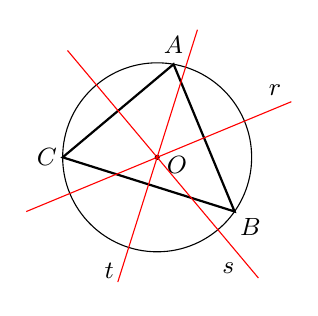
\begin{tikzpicture}[scale=0.6,font=\small]
\usetikzlibrary{calc}

\begin{scope}
%\clip (-2.1,-2.1) rectangle (2.5,2.1);
\coordinate (o) at (0,0);
\coordinate (a) at (80:2);
\coordinate (b) at (180:2);
\coordinate (c) at (325:2);

\draw (o) circle (2);

\draw[thick] (a) node[above] {$A$} -- (b) node[shift={(-0.2,0)}] {$C$} -- (c) node[shift={(0.2,-0.2)}] {$B$} -- cycle;
\draw[fill] (o) circle (1.2pt) node[shift={(0.25,-0.1)}] {$O$};
\draw[red, shorten >=-1.8cm,shorten <=-1.2cm] ($(a)!(o)!(c)$) node[black, shift={(0.9,0.6)}] {$r$} -- (o);
\draw[red, shorten >=-1.7cm,shorten <=-1.3cm] ($(b)!(o)!(c)$) node[black, shift={(-0.5,-1.1)}] {$t$} -- (o);
\draw[red, shorten >=-2cm,shorten <=-1cm] ($(a)!(o)!(b)$) node[black, shift={(1.4,-2)}] {$s$} -- (o);

\end{scope}

\end{tikzpicture}

\end{minipage}\vspace{5pt}

\noindent\begin{minipage}{0.7\textwidth}\parindent15pt
\begin{esercizio}[Prove invalsi 2007]
\label{ese:5.60}
Osserva la figura. Quale delle seguenti affermazioni è vera?
\begin{enumeratea}
\item Il triangolo è inscritto nella circonferenza minore.
\item Il triangolo è inscritto nella circonferenza maggiore.
\item La circonferenza maggiore è inscritta nel triangolo.
\item Il triangolo è circoscritto alla circonferenza maggiore.
\end{enumeratea}
\end{esercizio}
\end{minipage}\hfil
\begin{minipage}{0.3\textwidth}
	\centering% Copyright (c) 2015 Daniele Masini - d.masini.it@gmail.com

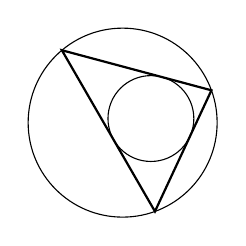
\begin{tikzpicture}[scale=0.6,font=\small]
\usetikzlibrary{calc}

\begin{scope}
\clip (-2.01,-2.01) rectangle (2.01,2.01);
\coordinate (o) at (0,0);
\coordinate (a) at (20:2);
\coordinate (b) at (130:2);
\coordinate (c) at (290:2);

\draw (o) circle (2);

\draw[thick] (a) -- (b) -- (c) -- cycle;
%\draw[fill] (o) circle (1.2pt) node[shift={(0.25,-0.1)}] {$O$};

\path (b) let \p1 = ($(a)-(b)$) in -- ($(b)!{veclen(\x1,\y1)}!(c)$) -- +($(a)-(b)$) coordinate (ob);
%\path (a) let \p1 = ($(b)-(a)$) in -- ($(a)!{-veclen(\x1,\y1)}!(c)$) -- +($(b)-(a)$) coordinate (oa);
%\coordinate (o) at (intersection of b--ob and a--oa);
\path (c) let \p1 = ($(a)-(c)$) in -- ($(c)!{veclen(\x1,\y1)}!(b)$) -- +($(a)-(c)$) coordinate (oc);
%\path (a) let \p1 = ($(c)-(a)$) in -- ($(a)!-{veclen(\x1,\y1)}!(b)$) -- +($(c)-(a)$) coordinate (ma);
%\coordinate (m) at (intersection of c--mc and a--ma);
%\coordinate (n) at (intersection of m--c and o--b);
\coordinate (oi) at (intersection of b--ob and c--oc);
\coordinate (h) at ($(b)!(oi)!(c)$);

\draw (oi) let \p1 = ($(oi)-(h)$) in circle ({veclen(\x1,\y1)});

\end{scope}

\end{tikzpicture}

\end{minipage}\vspace{5pt}

\noindent\begin{minipage}{0.65\textwidth}\parindent15pt
\begin{esercizio}[Prove invalsi 2002]
\label{ese:5.61}
Osserva la figura. I due angoli $A\widehat{C}B$ e $A\widehat{C'}B$ sono uguali? Quali sono le loro ampiezze in gradi?
\begin{enumeratea}
\item Non sono uguali e $A\widehat{C}B=90\grado$ e $A\widehat{C'}B=60\grado$
\item Non sono uguali e $A\widehat{C}B=60\grado$ e $A\widehat{C'}B=45\grado$
\item Sono uguali e $A\widehat{C}B=A\widehat{C'}B=60\grado$
\item Sono uguali e $A\widehat{C}B=A\widehat{C'}B=90\grado$
\item Sono uguali e $A\widehat{C}B=A\widehat{C'}B=180\grado$
\end{enumeratea}
\end{esercizio}
\end{minipage}\hfil
\begin{minipage}{0.35\textwidth}
	\centering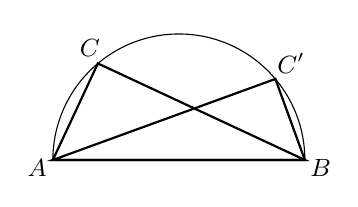
\begin{tikzpicture}[scale=0.8,font=\small]
\usetikzlibrary{calc}

\begin{scope}
\clip (-2.4,-0.3) rectangle (2.4,2.1);
\coordinate (o) at (0,0);
\coordinate (a) at (180:2);
\coordinate (b) at (0:2);
\coordinate (c) at (130:2);
\coordinate (c1) at (40:2);

\begin{scope}
\clip (-2.5,0) rectangle (2.5,2.5);
\draw (o) circle (2);
\end{scope}

\draw[thick] (a) node[shift={(-0.2,-0.1)}] {$A$} -- (b) node[shift={(0.2,-0.1)}] {$B$} -- (c) node[shift={(-0.1,0.2)}] {$C$} -- cycle;
%\draw[fill] (o) circle (1.2pt) node[shift={(0.25,-0.1)}] {$O$};
\draw[thick] (a) -- (b) -- (c1) node[shift={(0.2,0.2)}] {$C'$} -- cycle;

\end{scope}

\end{tikzpicture}

\end{minipage}\vspace{5pt}

\noindent\begin{minipage}{0.7\textwidth}\parindent15pt
\begin{esercizio}[Prove invalsi 2003]
\label{ese:5.62}
Nella figura seguente $O$ è il centro della circonferenza, $B$ un punto su di essa e $AC$ un suo diametro. Sapendo che $A\widehat{O}B=80\grado$, quanto vale $C\widehat{A}B-A\widehat{C}B$?
\begin{enumeratea}
\item $5\grado$
\item $10\grado$
\item $15\grado$
\item $20\grado$
\item $40\grado$
\end{enumeratea}
\end{esercizio}
\end{minipage}\hfil
\begin{minipage}{0.3\textwidth}
	\centering% (c) 2014 Daniele Masini - d.masini.it@gmail.com
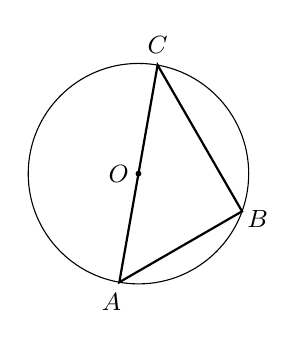
\begin{tikzpicture}[scale=0.7,font=\small]
\usetikzlibrary{calc}

\begin{scope}
%\clip (-2.1,-2.1) rectangle (2.5,2.1);
\coordinate (o) at (0,0);
\coordinate (a) at (260:2);
\coordinate (b) at (340:2);
\coordinate (c) at (80:2);

\draw (o) circle (2);

\draw[thick] (a) node[shift={(-0.1,-0.25)}] {$A$} -- (b) node[shift={(0.2,-0.1)}] {$B$} -- (c) node[shift={(0,0.25)}] {$C$} -- cycle;
\draw[fill] (o) circle (1.2pt) node[shift={(-0.25,0)}] {$O$};

\end{scope}

\end{tikzpicture}

\end{minipage}\vspace{5pt}

\begin{esercizio}[Prove invalsi 2003]
\label{ese:5.63}
Qual è il massimo numero di punti che una circonferenza e i quattro lati di un quadrato possono avere in comune?
\begin{multicols}{5}
\begin{enumeratea}
\item 2;
\item 4;
\item 6;
\item 8;
\item 10.
\end{enumeratea}
\end{multicols}
\end{esercizio}

\noindent\begin{minipage}{0.65\textwidth}\parindent15pt
\begin{esercizio}[Prove invalsi 2005]
\label{ese:5.64}
Osserva attentamente la figura. Sapendo che $A\widehat{O}B\cong C\widehat{O}D\cong B\widehat{V}C=\alpha$, quanto misura $A\widehat{O}D$?
\begin{multicols}{4}
\begin{enumeratea}
\item $\alpha$;
\item $2\alpha$;
\item $3\alpha$;
\item $4\alpha$.
\end{enumeratea}
\end{multicols}
\end{esercizio}
\end{minipage}\hfil
\begin{minipage}{0.35\textwidth}
	\centering% (c) 2014 Daniele Masini - d.masini.it@gmail.com
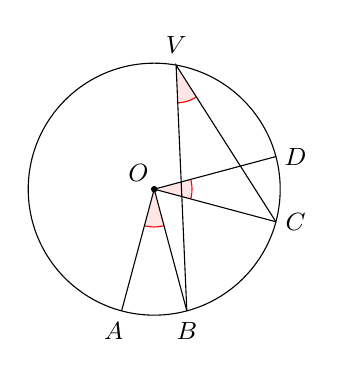
\begin{tikzpicture}[scale=0.8,font=\small]
\usetikzlibrary{calc}

\begin{scope}
%\clip (-2.1,-2.1) rectangle (2.5,2.1);
\coordinate (o) at (0,0);
\coordinate (a) at (255:2);
\coordinate (b) at (285:2);
\coordinate (c) at (-15:2);
\coordinate (d) at (15:2);
\coordinate (v) at (80:2);

\draw (o) circle (2);

\begin{scope}
\clip (a) -- (o) -- (b);
\draw[red, fill=red!10] (o) circle (0.6);
\end{scope}

\begin{scope}
\clip (c) -- (o) -- (d);
\draw[red, fill=red!10] (o) circle (0.6);
\end{scope}

\begin{scope}
\clip (b) -- (v) -- (c);
\draw[red, fill=red!10] (v) circle (0.6);
\end{scope}

\draw (a) node[shift={(-0.1,-0.25)}] {$A$} -- (o) -- (b) node[shift={(0,-0.25)}] {$B$};
\draw (c) node[shift={(0.25,0)}] {$C$} -- (o) -- (d) node[shift={(0.25,0)}] {$D$};
\draw (b) -- (v) node[shift={(0,0.25)}] {$V$} -- (c);
\draw[fill] (o) circle (1.2pt) node[shift={(-0.2,0.2)}] {$O$};

\end{scope}

\end{tikzpicture}

\end{minipage}\vspace{5pt}

\begin{esercizio}[Prove invalsi 2005]
\label{ese:5.65}
Qual è il massimo numero possibile di punti di intersezione fra una circonferenza e un triangolo?
\begin{multicols}{4}
\begin{enumeratea}
\item 6;
\item 5;
\item 4;
\item 3;
\end{enumeratea}
\end{multicols}
\end{esercizio}

\begin{esercizio}[Prove invalsi 2005]
\label{ese:5.66}
Quale delle seguenti affermazioni è falsa? 
\begin{enumeratea}
\item In ogni triangolo isoscele l'altezza e la mediana relative alla base e la bisettrice dell'angolo al vertice coincidono.
\item In ogni triangolo isoscele baricentro, incentro, ortocentro e circocentro sono allineati.
\item In ogni triangolo isoscele baricentro, ortocentro, incentro e circocentro coincidono.
\item In ogni triangolo equilatero baricentro, ortocentro, incentro e circocentro coincidono.
\end{enumeratea}
\end{esercizio}

\begin{esercizio}[Prove invalsi 2006]
\label{ese:5.67}
Considera la figura seguente. Se le due circonferenze hanno raggi diversi, quale delle seguenti affermazioni è vera?
\begin{enumeratea}
\item Le due circonferenze sono simmetriche rispetto al punto $O$.
\item Le due circonferenze sono simmetriche rispetto a ciascuna delle rette $r$ e $s$.
\item $AO_1:O_2C=OC:AO$.
\item $AO_1:O_2C=AO:OC$.
\end{enumeratea}
\end{esercizio}
\begin{figure}[!htb]
	\centering% (c) 2014 Daniele Masini - d.masini.it@gmail.com
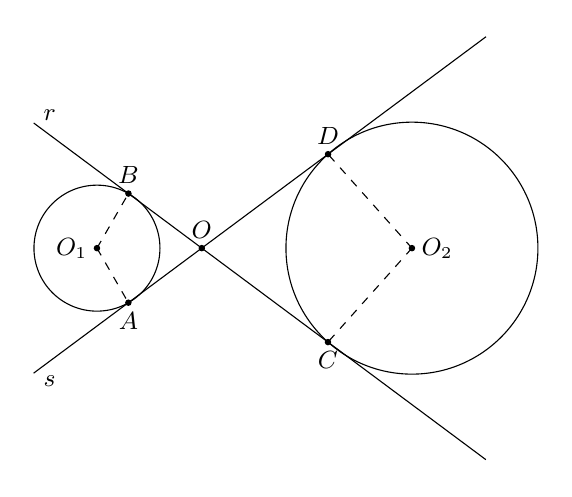
\begin{tikzpicture}[scale=0.8,font=\small]
\usetikzlibrary{calc,intersections}

\begin{scope}
\clip (-3.1,-3.5) rectangle (5.1,3.5);
\coordinate (o) at (0,0);
\coordinate (o1) at (-2,0);
\coordinate (o2) at (3,0);
\coordinate (m1) at ($(o1)!0.5!(o)$);
\coordinate (m2) at ($(o)!0.5!(o2)$);

\path[name path=Circle1] (m1) let \p1= ($(m1) - (o)$) in circle ({veclen(\x1,\y1)});
\path[name path=Circle2] (m2) let \p1= ($(m2) - (o)$) in circle ({veclen(\x1,\y1)});

\draw[name path=Circle3] (o1) circle (1);
\draw[name path=Circle4] (o2) circle (2);

\path [name intersections={of=Circle1 and Circle3}] ;
\draw[fill] (intersection-1) coordinate (b) node [above] {$B$} circle (1.2pt);
\draw[fill] (intersection-2) coordinate (a) node [below] {$A$} circle (1.2pt);
\path [name intersections={of=Circle2 and Circle4}] ;
\draw[fill] (intersection-1) coordinate (d) node [above] {$D$} circle (1.2pt);
\draw[fill] (intersection-2) coordinate (c) node [below] {$C$} circle (1.2pt);

\draw[shorten <=-1.5cm, shorten >=-2.5cm] (a) node[shift={(-1,-1)}] {$s$} -- (d);
\draw[shorten <=-1.5cm, shorten >=-2.5cm] (b) node[shift={(-1,1)}] {$r$} -- (c);

\coordinate (o3) at (intersection of a--d and b--c);

\draw[fill] (o3) circle (1.2pt) node[above] {$O$};
\draw[fill] (o1) circle (1.2pt) node[left] {$O_1$};
\draw[fill] (o2) circle (1.2pt) node[right] {$O_2$};

\draw[dashed] (o1) -- (a);
\draw[dashed] (o1) -- (b);
\draw[dashed] (o2) -- (c);
\draw[dashed] (o2) -- (d);

\end{scope}

\end{tikzpicture}

\end{figure}

\noindent\begin{minipage}{0.65\textwidth}\parindent15pt
\begin{esercizio}
\label{ese:5.68}
Nella figura seguente il punto $O$ è il punto medio del diametro $AC$. L'angolo $A\widehat{O}B$ misura $40\grado$. Quanto misura l'angolo $O\widehat{B}C$? 
\begin{multicols}{4}
\begin{enumeratea}
\item $10\grado$;
\item $20\grado$;
\item $40\grado$;
\item $60\grado$.
\end{enumeratea}
\end{multicols}
\end{esercizio}
\end{minipage}\hfil
\begin{minipage}{0.35\textwidth}
	\centering% (c) 2014 Daniele Masini - d.masini.it@gmail.com
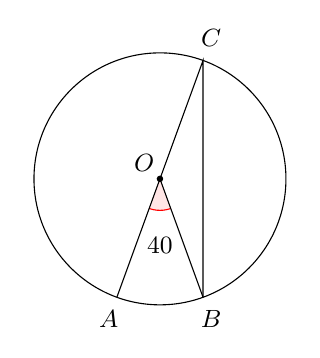
\begin{tikzpicture}[scale=0.8,font=\small]
\usetikzlibrary{calc}

\begin{scope}
\clip (-2.1,-2.4) rectangle (2.1,2.4);
\coordinate (o) at (0,0);
\coordinate (a) at (250:2);
\coordinate (b) at (290:2);
\coordinate (c) at (70:2);

\begin{scope}
\clip (a) -- (o) -- (b) -- cycle;
\draw[red, fill=red!10] (o) circle (0.5);
\node at (270:1.05) {$40\grado$};
\end{scope}

\draw[fill] (o) circle (1.2pt) node[shift={(-0.2,0.2)}] {$O$};

\draw (a) node [shift={(250:0.3)}] {$A$} -- (c) node [shift={(70:0.3)}] {$C$} -- (b) node [shift={(290:0.3)}] {$B$};
\draw (o) -- (b);

\draw (o) circle (2);

\end{scope}

\end{tikzpicture}

\end{minipage}\vspace{5pt}


\subsection{Risposte}

\begingroup
\hypersetup{linkcolor=black}

\paragraph{\ref{ese:5.5}.}
a)~F,\quad b)~V,\quad c)~F,\quad d)~V,\quad e)~V,\quad f)~V,\quad g)~V,\quad h)~F,\quad i)~V,\quad j)~V.

\paragraph{\ref{ese:5.60}.}
b.

\paragraph{\ref{ese:5.61}.}
d.

\paragraph{\ref{ese:5.62}.}
b.

\paragraph{\ref{ese:5.63}.}
d.

\paragraph{\ref{ese:5.64}.}
d.

\paragraph{\ref{ese:5.65}.}
a.

\paragraph{\ref{ese:5.66}.}
a.

\paragraph{\ref{ese:5.67}.}
d.

\paragraph{\ref{ese:5.68}.}
b.

\endgroup


\cleardoublepage
